\section{Analysis selection and efficiencies}
This section describes details of the event selection, reconstruction,
and trigger efficiencies. We first define acceptance selections that
ensure well-understood and high-efficiency reconstruction and
triggering, and then determine the efficiency of offline and trigger
selections for events satisfying acceptance cuts. We then discuss
modeling of the shape of the signal invariant mass distribution that
will be later be used in the fit and the systematics associated with
the accuracy of this shape.

\subsection{Minimal Acceptance Definition}
\label{sec:acceptance}
To avoid introducing complicated model-dependent efficiencies, signal
regions are defined by kinematic cuts that avoid trigger turn-on
curves and regions where detector effects lead to diminished trigger
or reconstruction efficiency. The latter becomes an issue when two or
more muons are very close to one another in the muon system.  Offline,
we use an arbitrated, inside-out muon identification algorithm that
minimizes such efficiency losses, discussed further in the text.  An
event satisfies minimal acceptance requirements if it passes the
following selections:
\begin{itemize}
\item at least one reconstructed muon candidate with $p_T >
  15$~GeV/$c$ and $|\eta| < 0.9$ per event (ensures high and
  well-understood trigger efficiency, see Sec.~\ref{sec:trig_selections});
\item at least one additional muon candidate with $p_T > 5$~GeV/$c$
  and $|\eta| < 2.4$ (ensures high and well-understood reconstruction
  efficiency).
\end{itemize}
Events satisfying minimal acceptance requirements are preserved for
further analysis and categorization. Additional muon candidates, if
present in the event, are used only if they also satisfy the $p_T >
5$~GeV/$c$ and $|\eta| < 2.4$ requirements.

\subsection{Reconstruction and Efficiency}
\label{sec:reconstruction_and_efficiency}

Muons in this analysis are identified by matching tracks in the inner
tracker to segments reconstructed in the muon chambers (inside-out),
arbitrated such that tracks and segments are used only once.  The muon
reconstruction algorithm used in many other CMS analyses require a
multi-segment muon track to be built in the muon chambers and then
matched to a track in the inner tracker (outside-in), but the low
segment multiplicity and large multiple scattering in the CMS magnet
return yoke makes this method inefficient for muons whose trajectories
cross each other in the muon system (as low as 50\%, see
Appendix~\ref{sec:motivation_for_reconstruction_methods}).  While this
inefficiency is undesirable in itself, it is especially problematic
for a model-independent analysis, because different models can predict
different distributions of muon trajectory overlaps, which would make
it impossible to apply a single efficiency correction to all cases.
The inside-out muon identification used in this analysis, however,
is much less sensitive to this source of inefficiency.

\subsubsection{Effects Related to the Muon System and Matching}
To ensure a high-purity muon sample, we additionally require every
muon to have at least two arbitrated segments\footnote{Arbitration in this case 
refers to the requirement that a given muon segment can be assigned to only
one tracker track, the assignment is done by considering all potential matches
among tracker tracks and choosing the most compatible one}, at least eight tracker
hits, and a tracker-track $\chi^2/N_{\mbox{\scriptsize DOF}} < 4$.
Although the cut on arbitrated segments re-introduces a dependence on
whether the muon trajectories cross in the muon system, this
inefficiency is still much less severe than the outside-in algorithm.
The arbitrated segments cut also eliminates as many fake muons from
accidental overlaps and punch-through as the outside-in algorithm.

An overview of muon reconstruction efficiency with the above algorithm
and cuts is presented in Fig.~\ref{fig:recoefficiency}.  A Monte Carlo
sample of dimuons is generated with flat distributions in dimuon mass
and vector-sum $p_T$ and $\eta$, passed through the full CMS detector
simulation, and is subject to the same reconstruction algorithms and
cuts as data.  The sample is partitioned into ``crossing'' muons and
``non-crossing'' muons by discriminating on angular distance between
the muons at a given depth in the muon system.\footnote{$\Delta \phi$
  = difference in azimuthal angle of the two muon trajectories, each
  evaluated on a cylinder centered on the beamline with 600~cm radius
  for $|\eta| < 1$ and one of two transverse planes, 700~cm from the
  interaction point, for $|\eta| > 1$.  Crossing muons have $\Delta
  \phi < 0.3$~mrad and non-crossing muons have $\Delta \phi >
  0.3$~mrad.  (See
  Appendix~\ref{sec:motivation_for_reconstruction_methods} for
  details.)}  Figure~\ref{fig:recoefficiency} presents three
efficiencies: (a)~the probability of reconstructing at least one muon,
(b)~the probability of reconstructing a specific muon (the leading
muon), and (c)~the probability of reconstructing both muons: (c) is
approximately the square of (b), as expected.  Inefficiency for
crossing muons is maximal for high-momentum and very forward muons,
where trajectories are nearly straight and collinear, allowing for
confusion between the candidate muon segments.  However, this
difference in efficiency reaches an extreme value of only 7\% at
$|\eta| = 2.4$, and is only 2\% for a distribution uniform in $\eta$.

\begin{figure}[tbh]
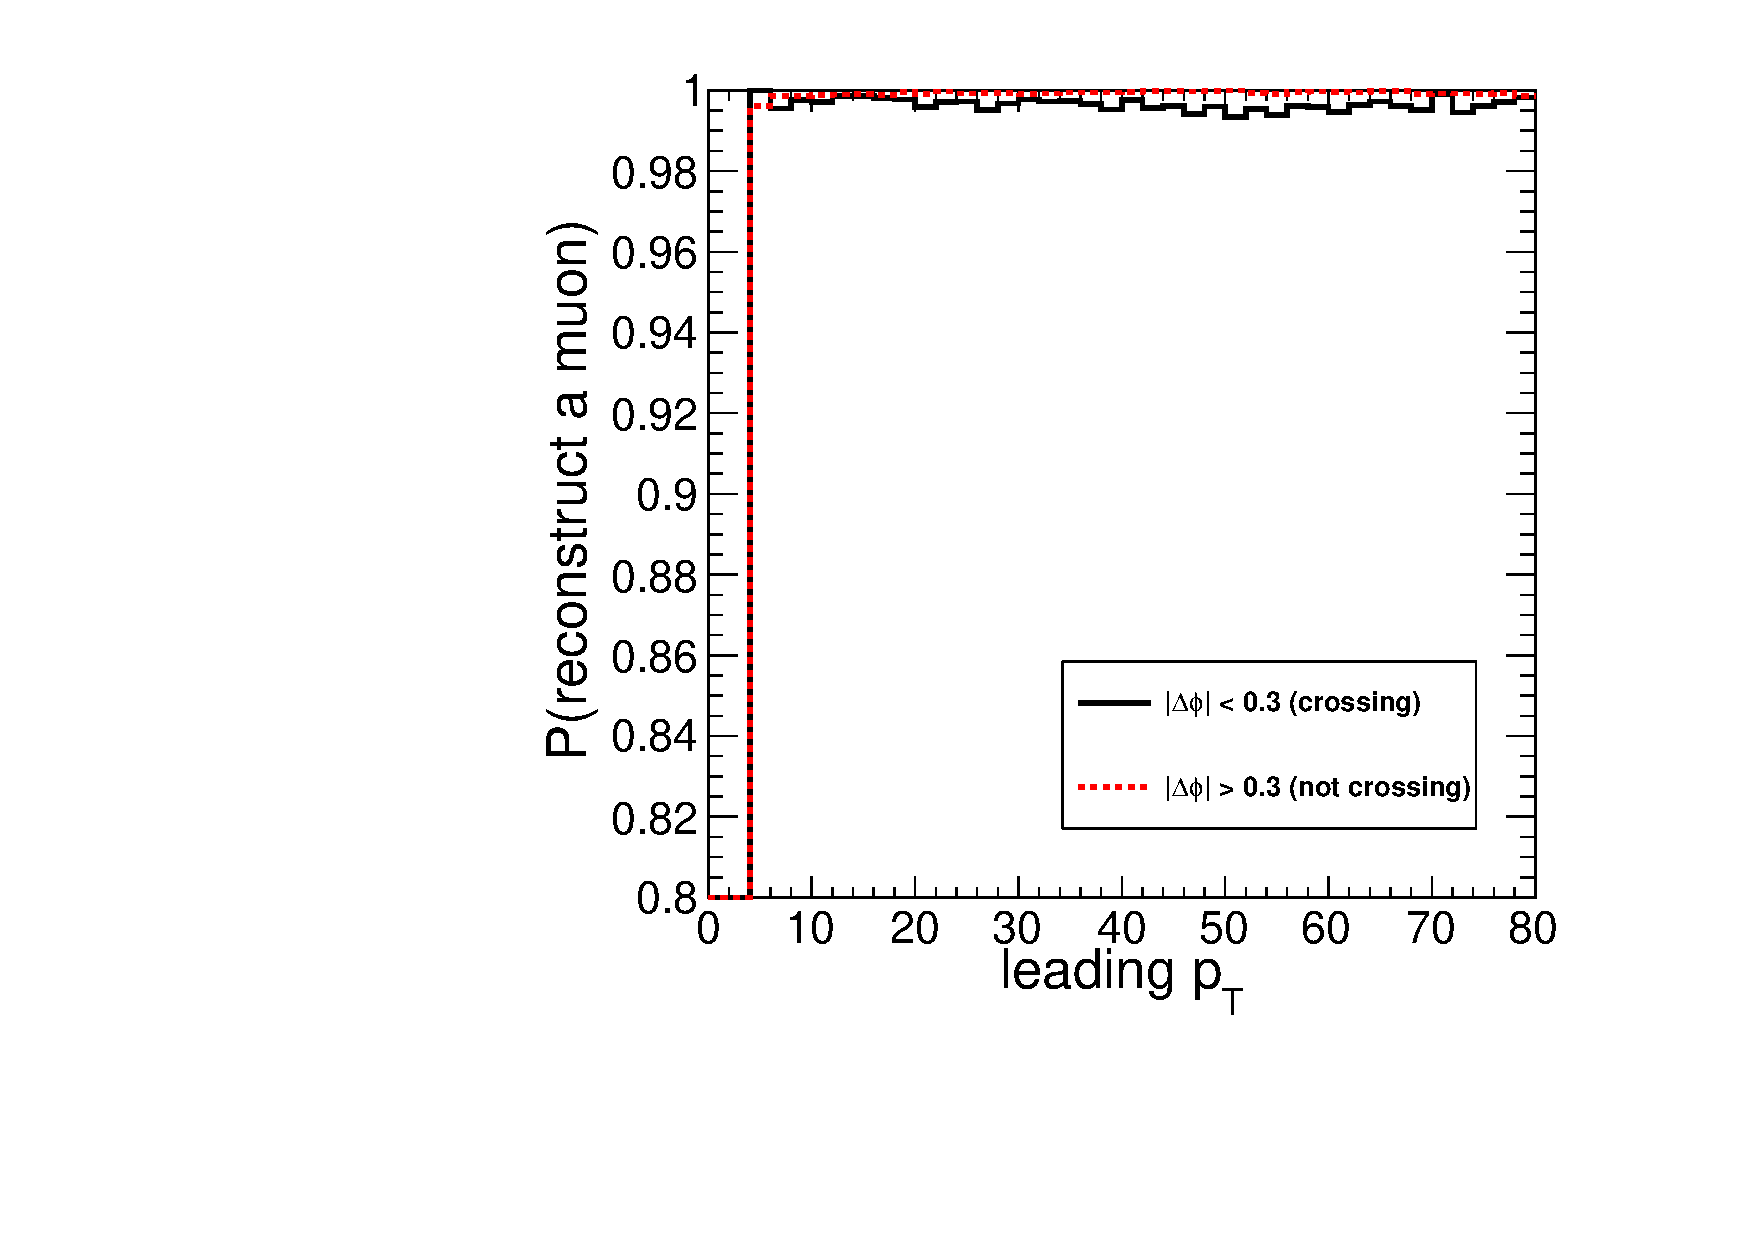
\includegraphics[width=0.32\linewidth]{PLOTS/pt_mass5cut_oneTrackerMuon.pdf} \hfill
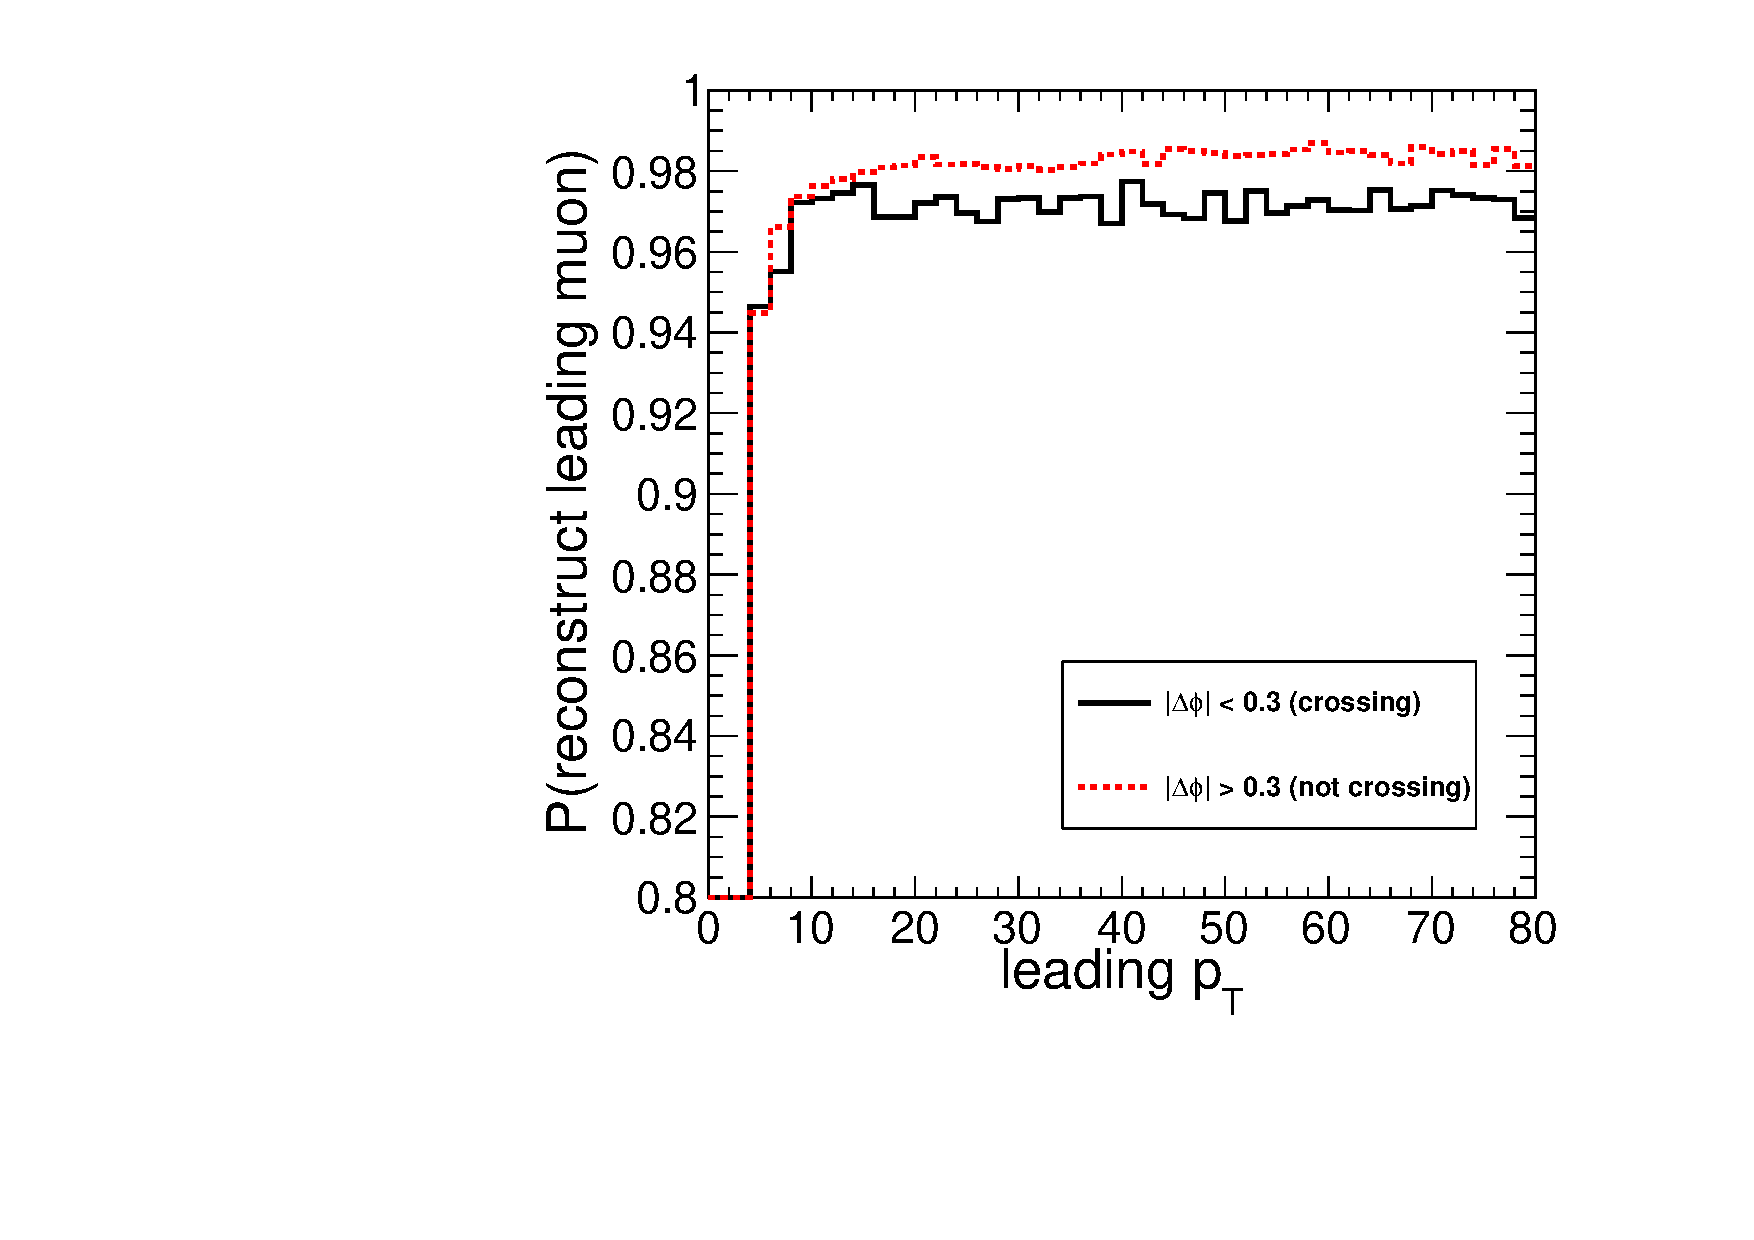
\includegraphics[width=0.32\linewidth]{PLOTS/pt_mass5cut_leadingTrackerMuon.pdf} \hfill
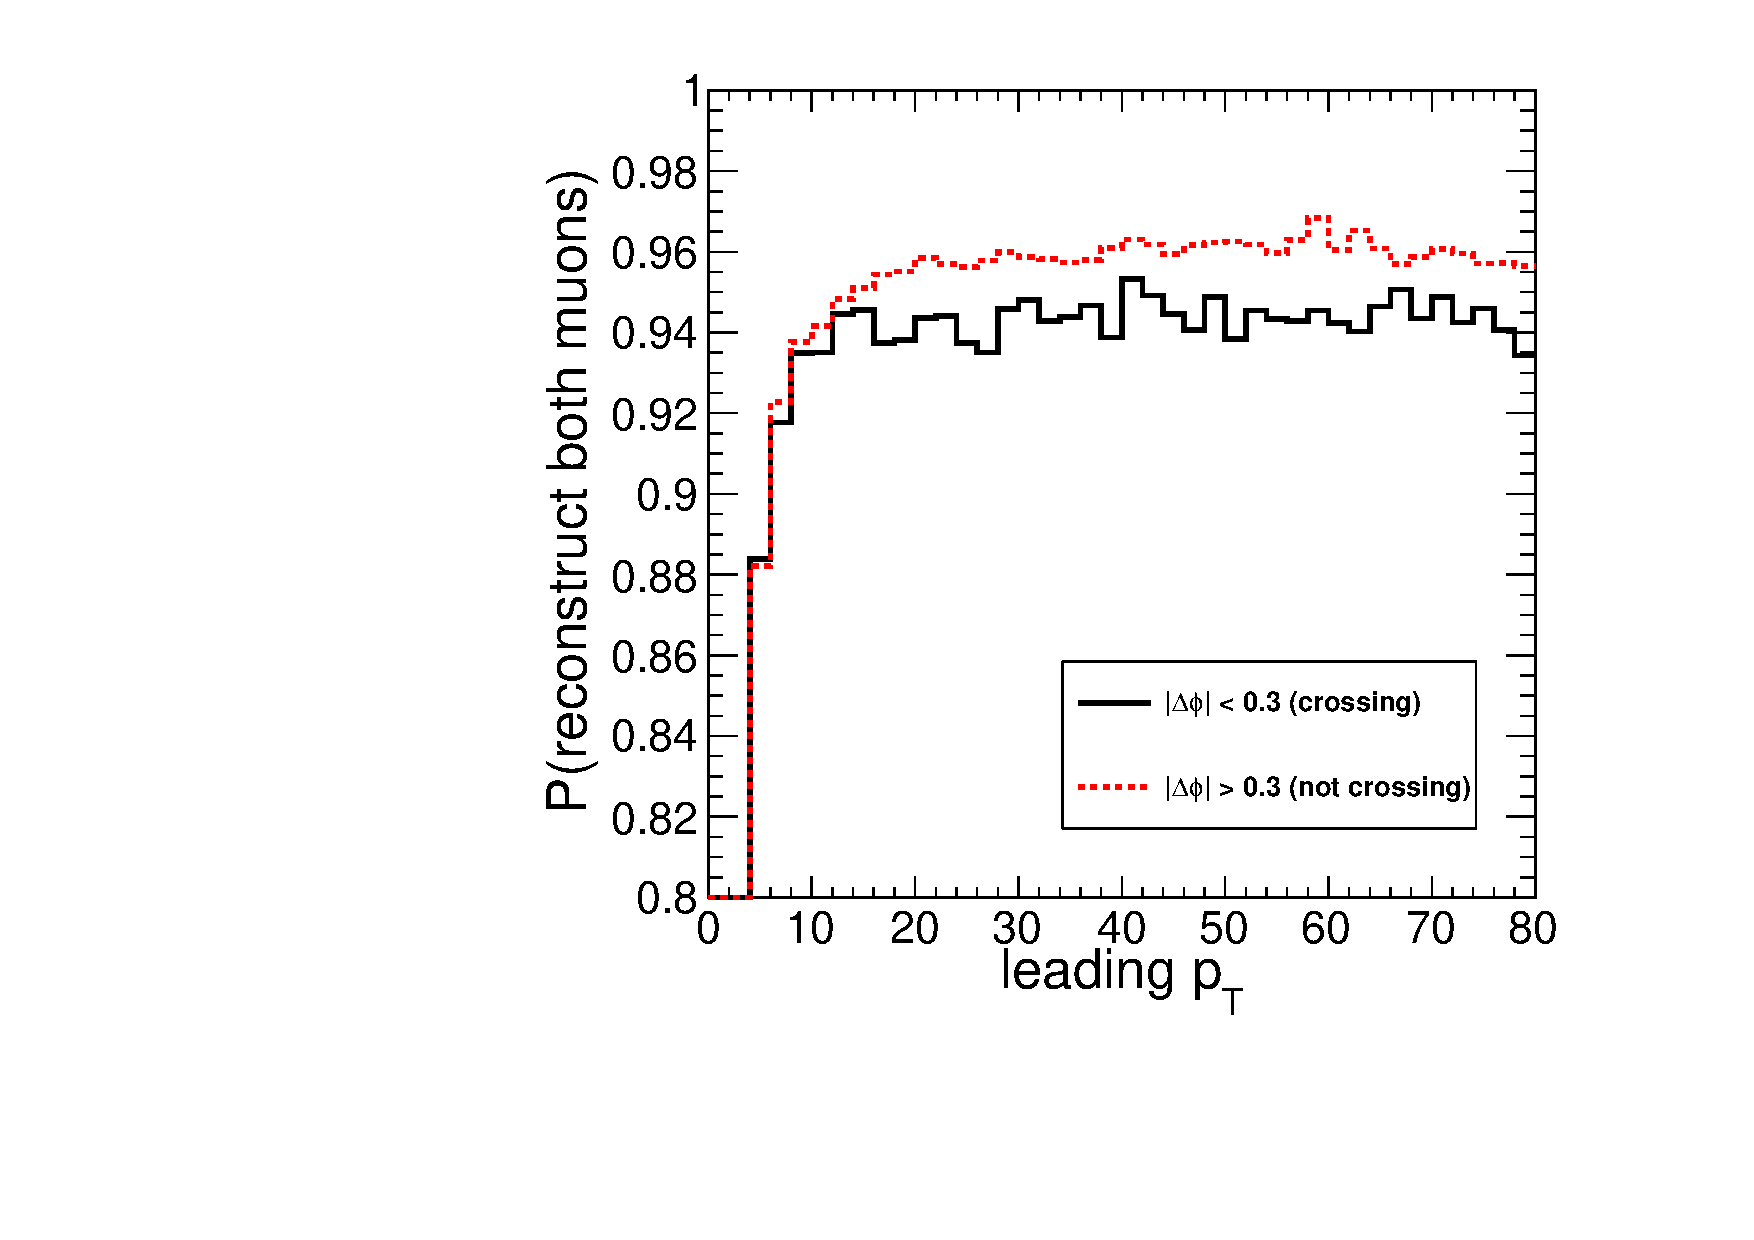
\includegraphics[width=0.32\linewidth]{PLOTS/pt_mass5cut_twoTrackerMuons.pdf}

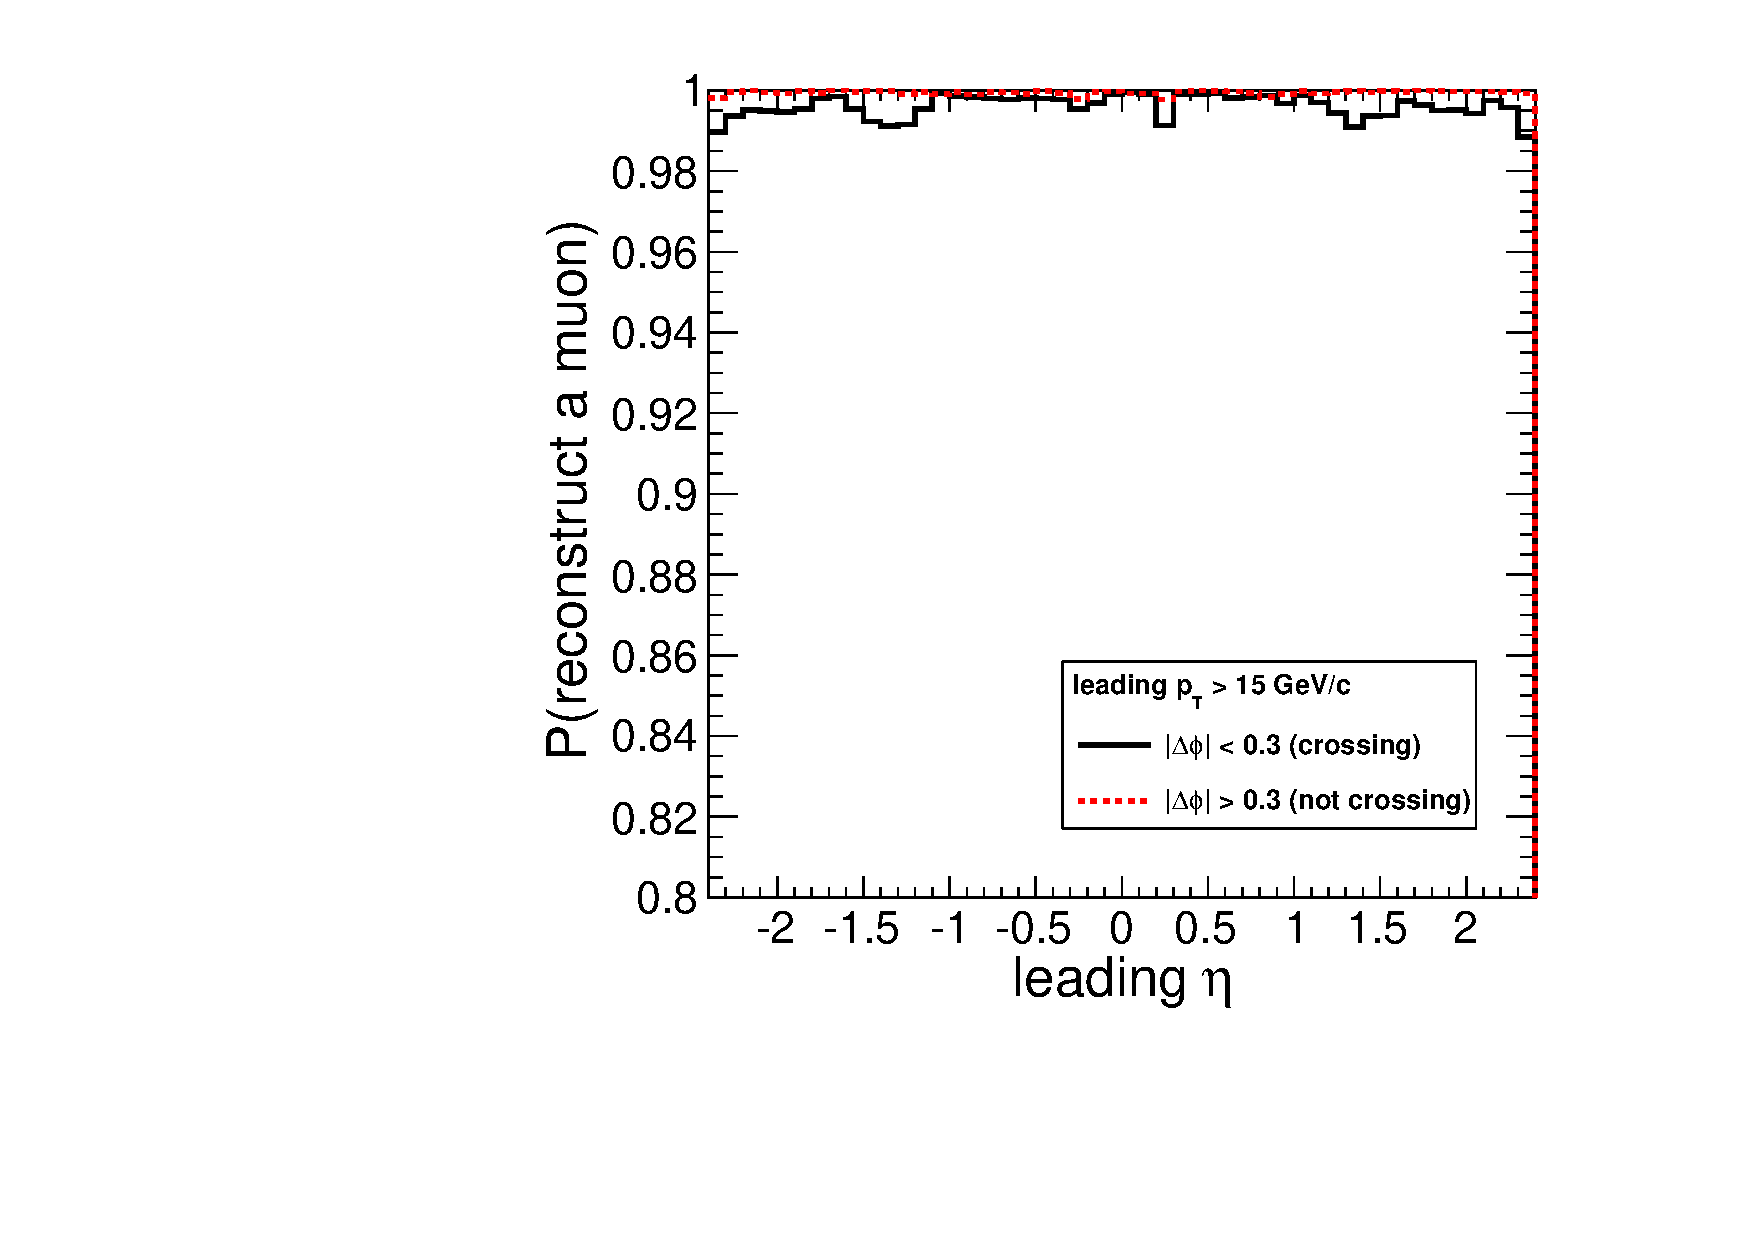
\includegraphics[width=0.32\linewidth]{PLOTS/eta_mass5cut_oneTrackerMuon.pdf} \hfill
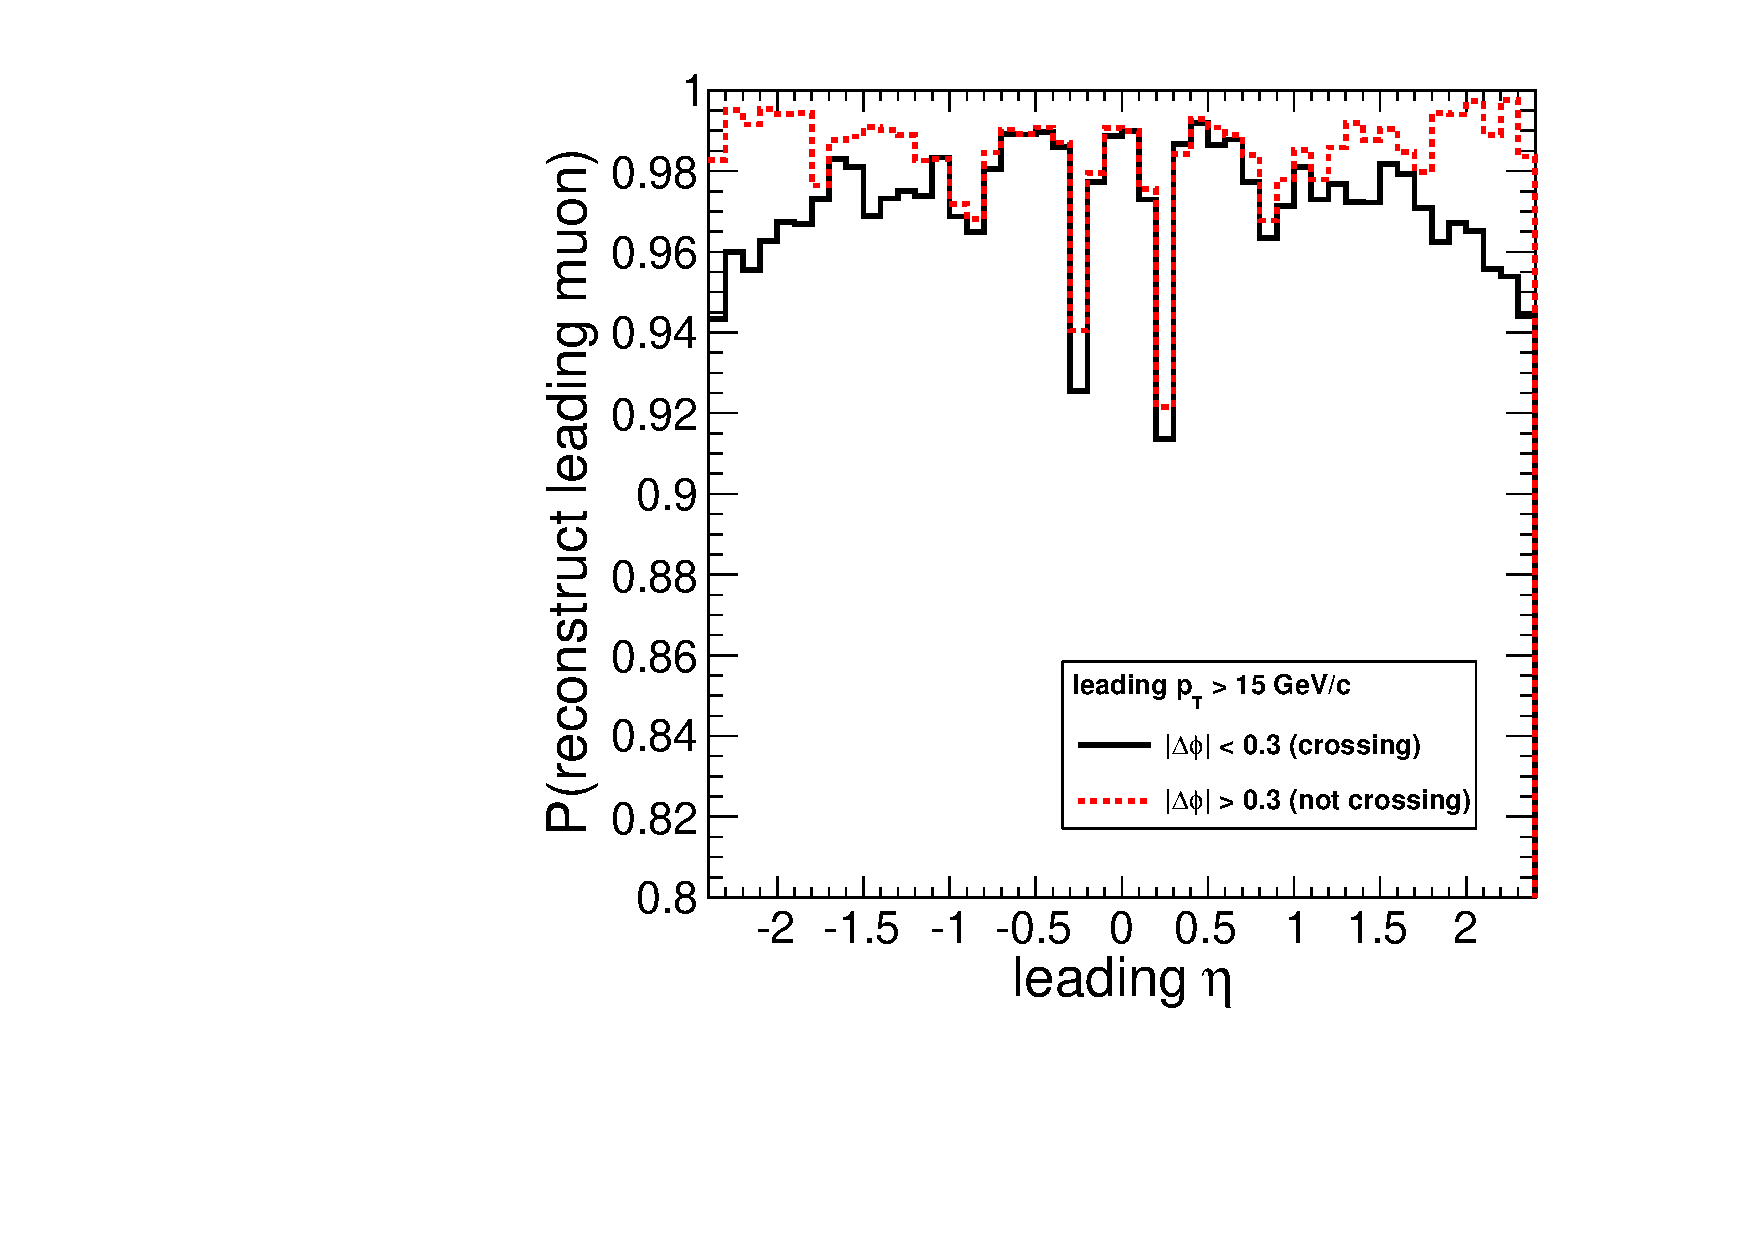
\includegraphics[width=0.32\linewidth]{PLOTS/eta_mass5cut_leadingTrackerMuon.pdf} \hfill
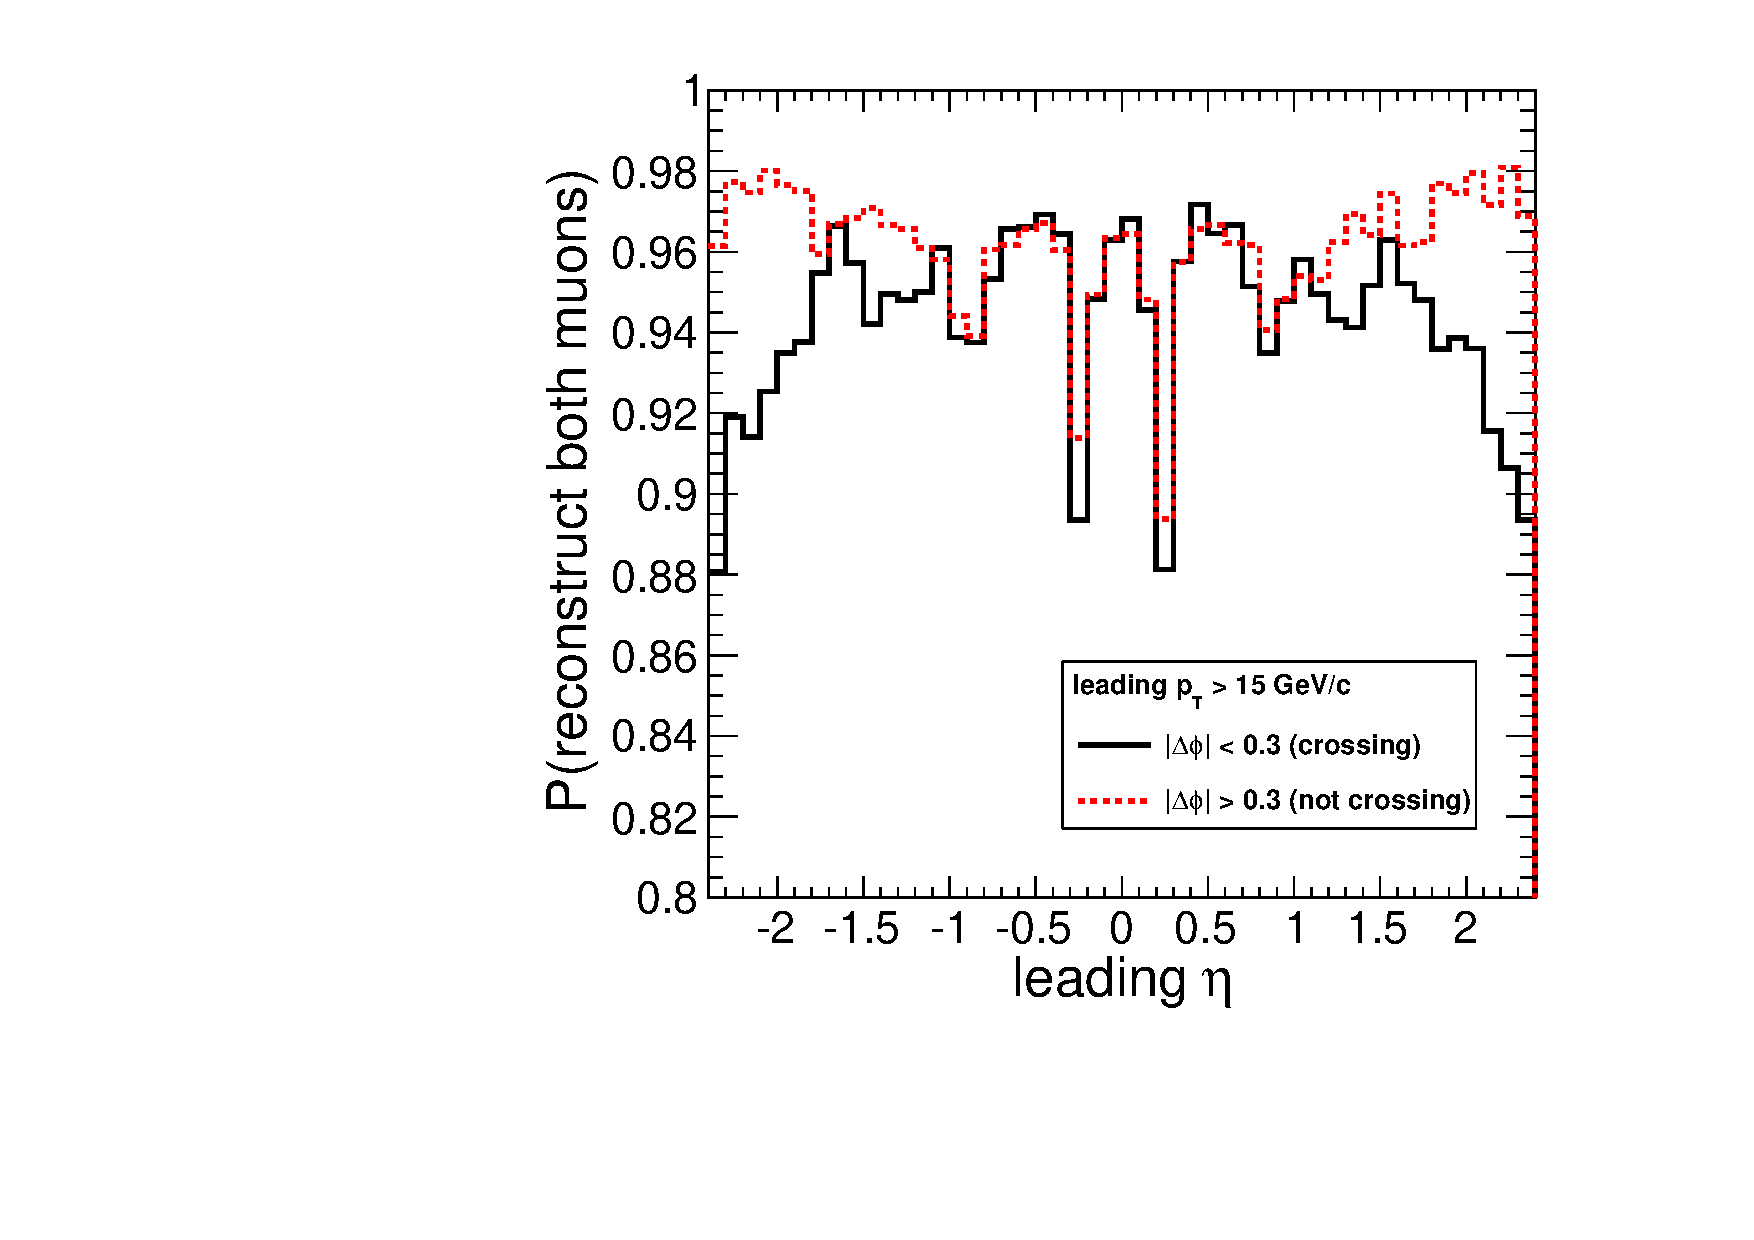
\includegraphics[width=0.32\linewidth]{PLOTS/eta_mass5cut_twoTrackerMuons.pdf}

\caption{Reconstruction efficiency as a function of momentum (top) and
  pseudorapidity (bottom), depending on whether the muon trajectories
  cross in the muon system.  All muons in this sample have $p_T >
  5$~GeV/$c$ and $|\eta| < 2.4$, and the pseudorapidity plots have at
  least one muon with $p_T > 15$~GeV/$c$ (see text for details). \label{fig:recoefficiency}}
\end{figure}

Acceptance corrections for each signal region are calculated in
Sec.~\ref{sec:complete_acceptance} using realistic benchmark models.
A systematic uncertainty of 1.3\% (the difference in single-muon
efficiency between the crossing and non-crossing cases) is applied to
each $|\eta| < 2.4$ muon, to account for the unknown fraction of
overlapping trajectories in the general case.  No such uncertainty is
applied for $|\eta| < 0.9$ muons. Apart from the collective effects
related to crossing trajectories, the single muon reconstruction efficiency 
is high (of the order of 97-98\% efficient, see Fig.~\ref{fig:recoefficiency}(b)) and 
is known to about 0.3\% per muon. We apply this systematics uncertainty for 
each reconstructed muon. While the overall per muon efficiency is high, the 
efficiency for reconstructing a very narrow group of muons has a correlated
term due to the dips in efficiency in the gaps between the wheels (the structure 
in $\eta$ seen in Figs.~\ref{fig:recoefficiency}(e) and (f)). if a narrow muon
jets crosses one of these gap regions, the efficiency of reconstructing each
muon crossing the gap region is substantially lower (of the order of 92\% per 
muon). Because the efficiency in the gaps is determined by the accuracy in describing
the fiducial volumes of the muon chambers, we assign an additional uncertainty of 
1\% for every muon in the gap region, which corresponds to a 10\% uncertainty
in the accuracy with which simulation describes the size of the gap (corresponds to
about 2 cm, the gap size is about 25 cm). Summarizing, the efficiency and its
uncertainty for a group of $N$ muons in the barrel approximately follows 
$\epsilon = (0.970 \pm 0.003)^{n_1} \times (0.92 \pm 0.01)^{n_2}$, where 
$n_1$ is the number of muons not crossing the gap and $n_2$ is the number of muons 
in the group that cross the gap ($n_1+n_2=N$).

\subsubsection{Effects Related to Muon Track Reconstruction in the Tracker}
For very high momentum muon groups, there is an additional inefficiency associated with
the cases when closeness of the track trajectories in the tracker results in one of the
tracks not being reconstructed. More precisely, a track is not reconstructed if it shares 
more than 50\% of its hits with other tracks. For reference, with the cluster sizes of the 
order of 1-2 channels (pixels or strip widths in $r-\phi$) for nearly straight tracks, two
opposite sign tracks with $p_T>300$ GeV/c and nearly parallel at the origin will be within
about 1 pixel/strip of each other up to the radius of 60 cm (TOB) acquiring very significant
efficiency losses due to hit sharing. While models with such high momentum muon pairs are 
outside of the kinematic reach of this analysis, tracking inefficiency is not negligible for
higher momentum muon jets ($p_T\sim 100-300$ GeV/c per group) that may be currently 
accessible. Because this kinematic limit is per muon group, muon pairs are the most affected 
at given muon jet $p_T$ as for higher multiplicity muon jets the momentum is shared 
between multiple muons leading to the lower average muon momenta and decreasing
the probability of significant overlaps. E.g. the tracking inefficiency in a quadmuon from 
$h_d \to \gamma_d \gamma_d \to 4 \mu$ is generally driven by the inefficiency in 
reconstructing the muon pair of higher momentum.

To demonstrate effects of tracking efficiency, Fig.~\ref{fig:highpttrackingstudy_kinematics} shows
step-by-step efficiency of reconstructing a pair of muons as a function of $p_T$ of the pair, invariant
mass of the pair and $\eta$ for pairs generated using a pair gun with a flat distribution in $p_T(\mu \mu)=0-500$
GeV/c, invariant mass $m=2m(\mu)-0.6$ and $\eta=-0.9-0.9$.  Ignoring the kinematic thresholds in 
reconstructing the sample and the unavoidable averaging over non-physical distributions in the sample,
it is evident that the $p_T$ dependent effects are driven by the tracker. The shape of the efficiency
as a function of the invariant mass is determined by the differences in efficiencies for the ``cowboy''
(the two tracks bend towards each other in the tracker) and ``sailor'' (the two tracks bend away 
from each other) topologies. Depending on the mass and momentum of the pair, tracks in the 
``cowboy'' topology can remain close throughout a substantial portion of the the tracker volume
leading to reduced efficiency. For very small masses ($m(\mu\mu)\sim2m(\mu)$), the difference
between the two becomes small as the two tracks are nearly parallel at the origin. Additional and more detailed
studies are presented in Appendix~\ref{appendix-high-boost-dimuon-efficiency}. Because closeness 
of the two tracks depends both on the invariant mass and the momentum of the pair, a convenient way
to present tracking efficiency is to plot it as a function of Lorentz boost $\gamma=p(\mu\mu)/m(\mu\mu)$ 
shown in Fig.~\ref{fig:highpttrackingstudy_kinematics}(d). The increase in the efficiency at high $\gamma$ 
is because that region is populated by pairs with high momentum and low invariant mass $m(\mu\mu)<0.3$ GeV/c 
where the two tracks are nearly parallel, in which case the tracks in the ``cowboy'' topology at the origin intersect 
at smaller radii and frequently become effectively ``sailors'' in the tracker. Generally, the onset of inefficiency 
starts earlier in $p_T(\mu\mu)$ for ``cowboys'' than for ``sailors'' as at a fixed momentum tracks in the ``cowboy'' 
topology tend to stay close longer.

\begin{figure}
\begin{center}
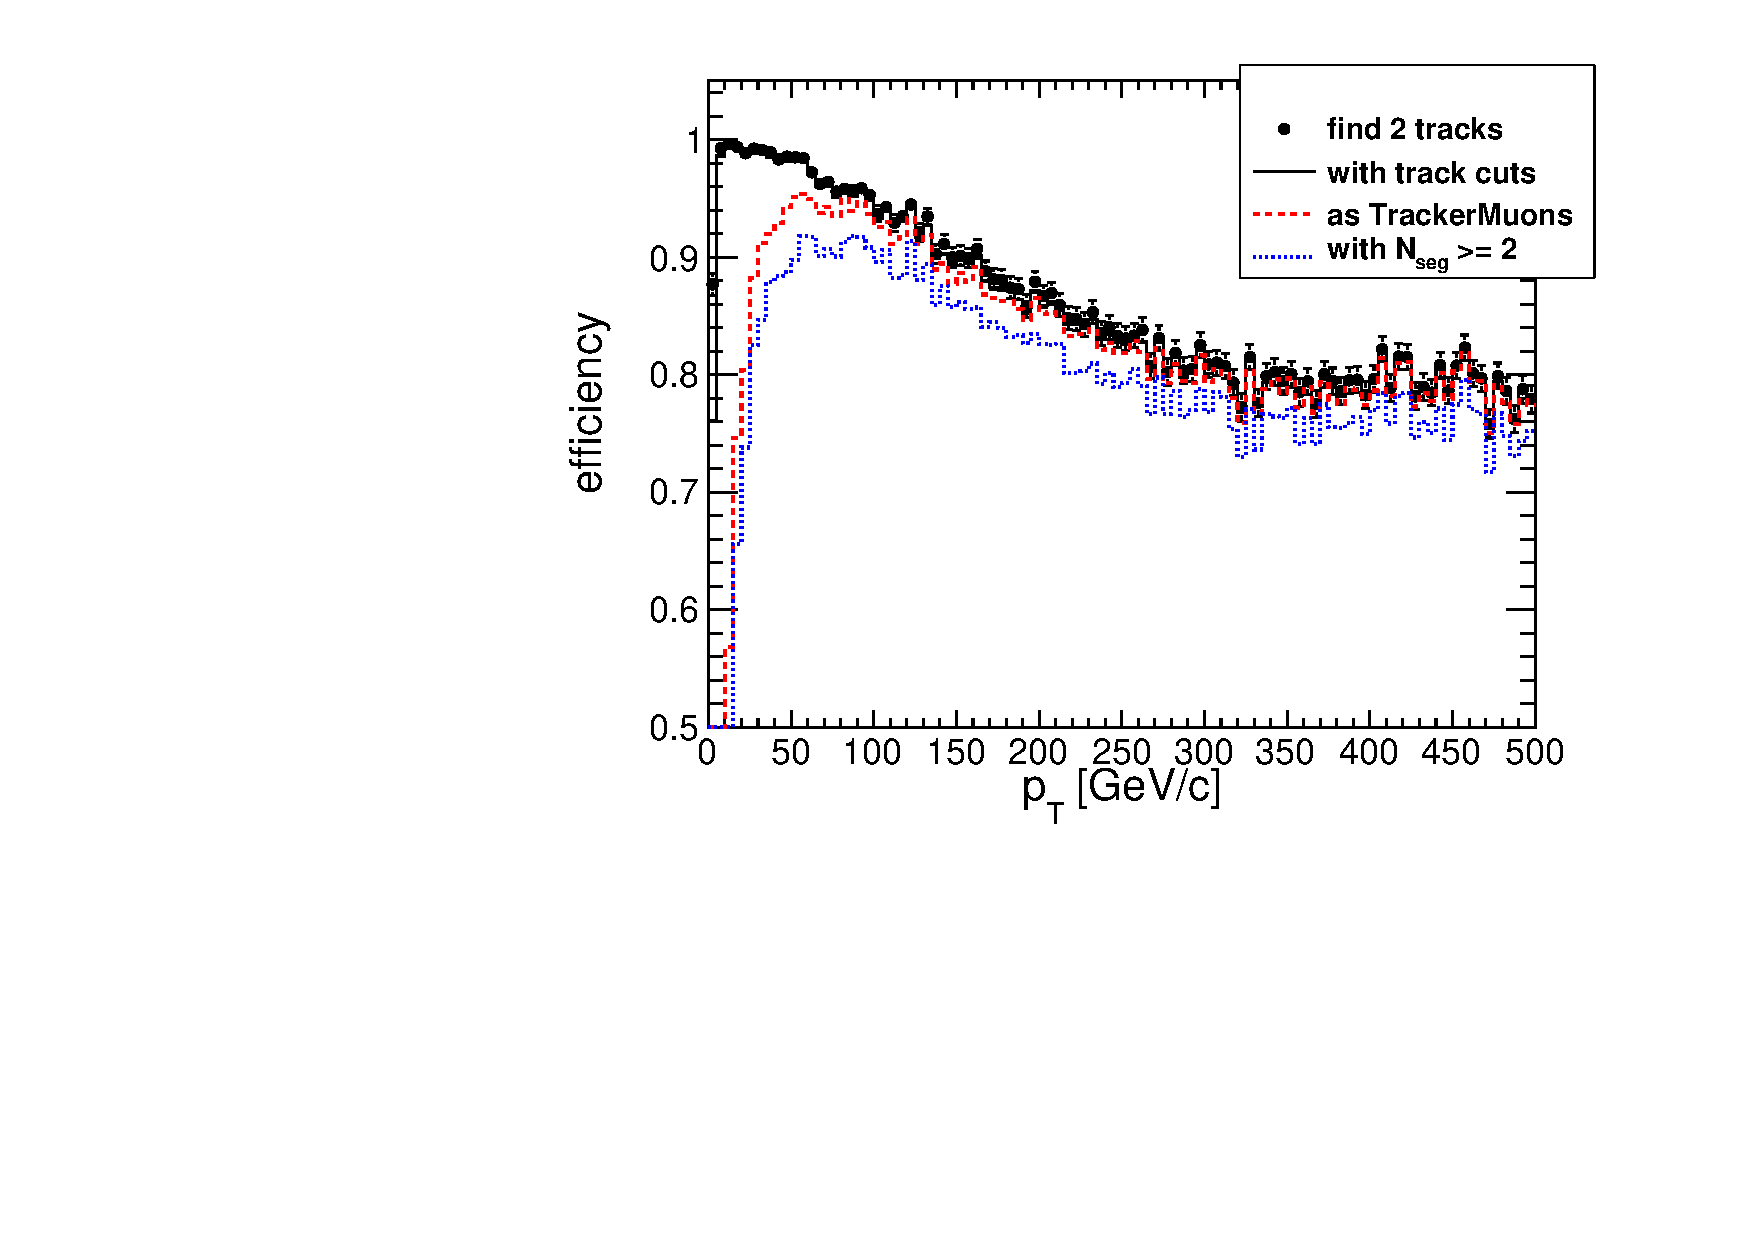
\includegraphics[width=0.48\linewidth]{PLOTS/HIGHPT_STUDY/highptstudy_pt.pdf} \hfill
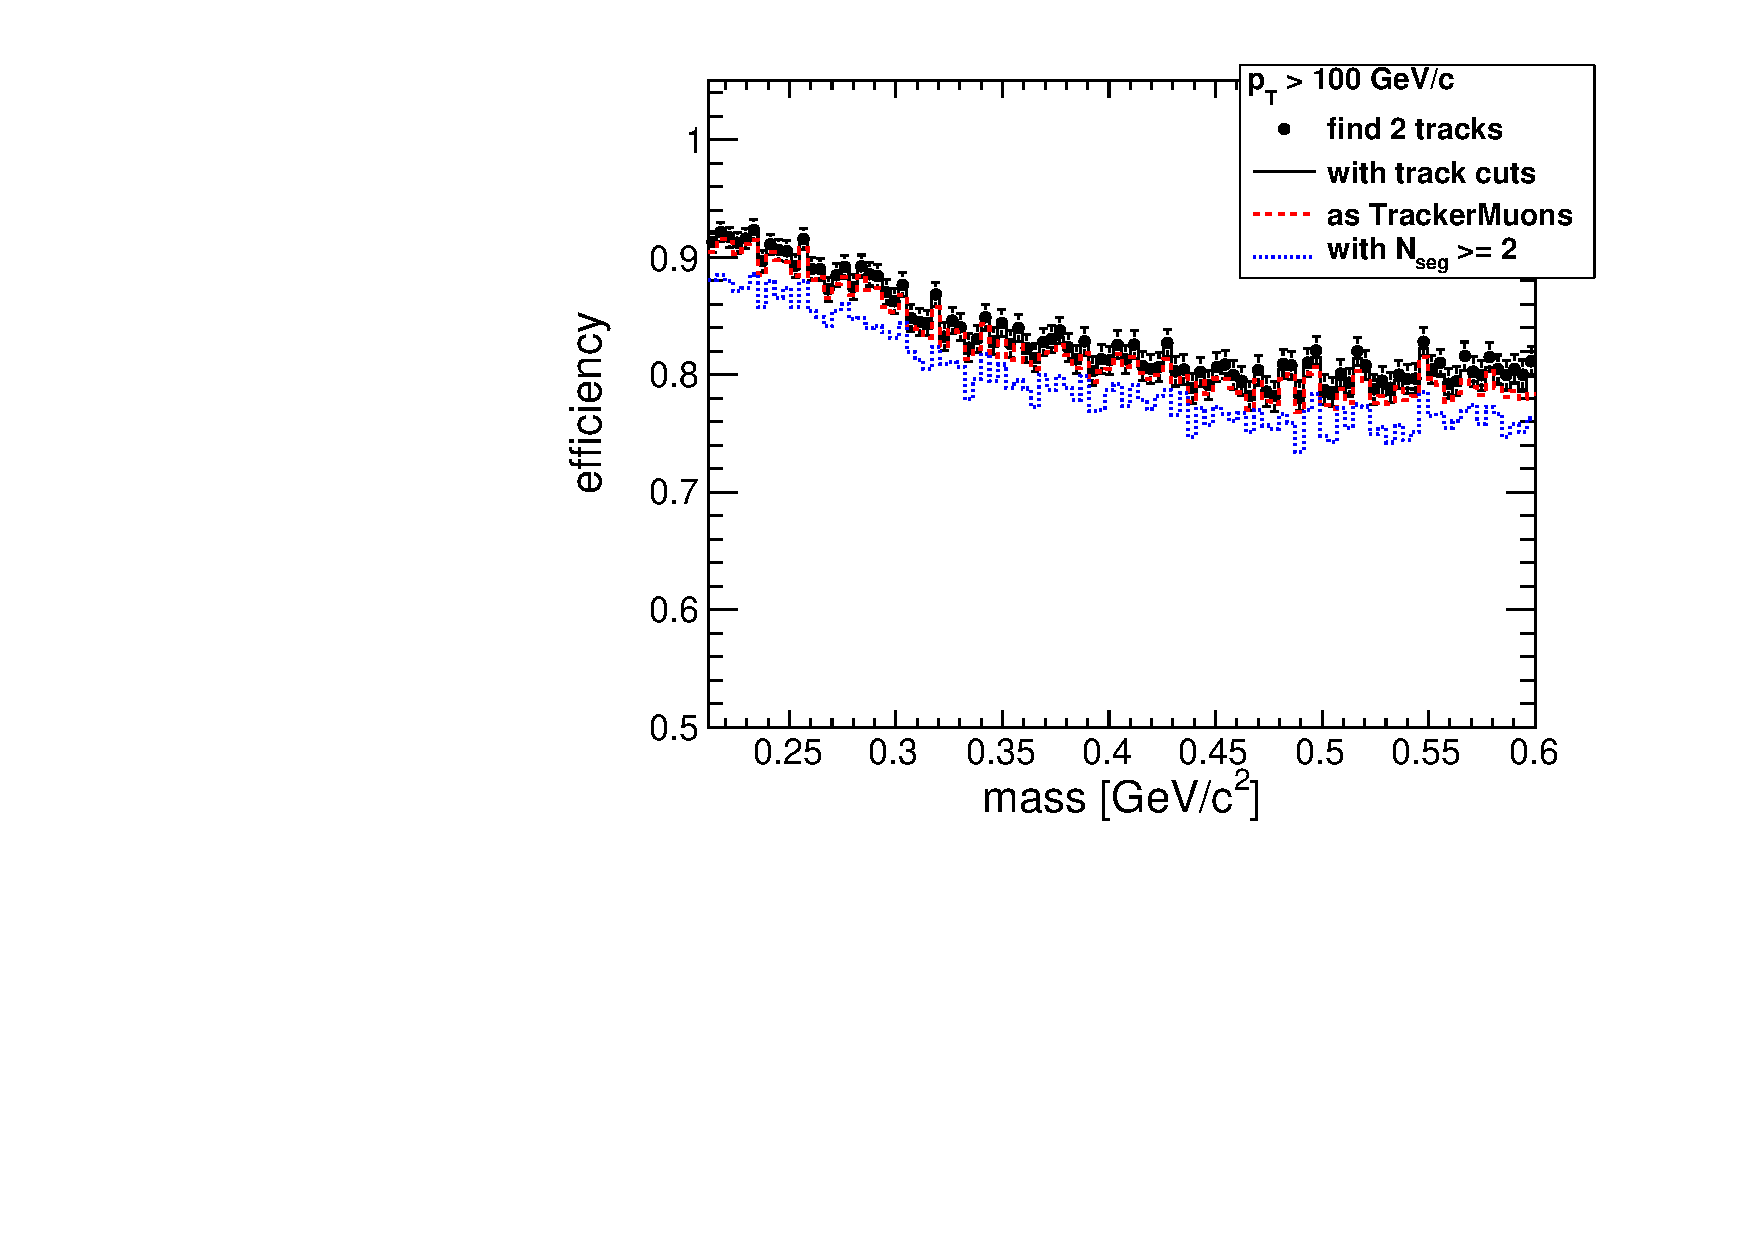
\includegraphics[width=0.48\linewidth]{PLOTS/HIGHPT_STUDY/highptstudy_mass.pdf}
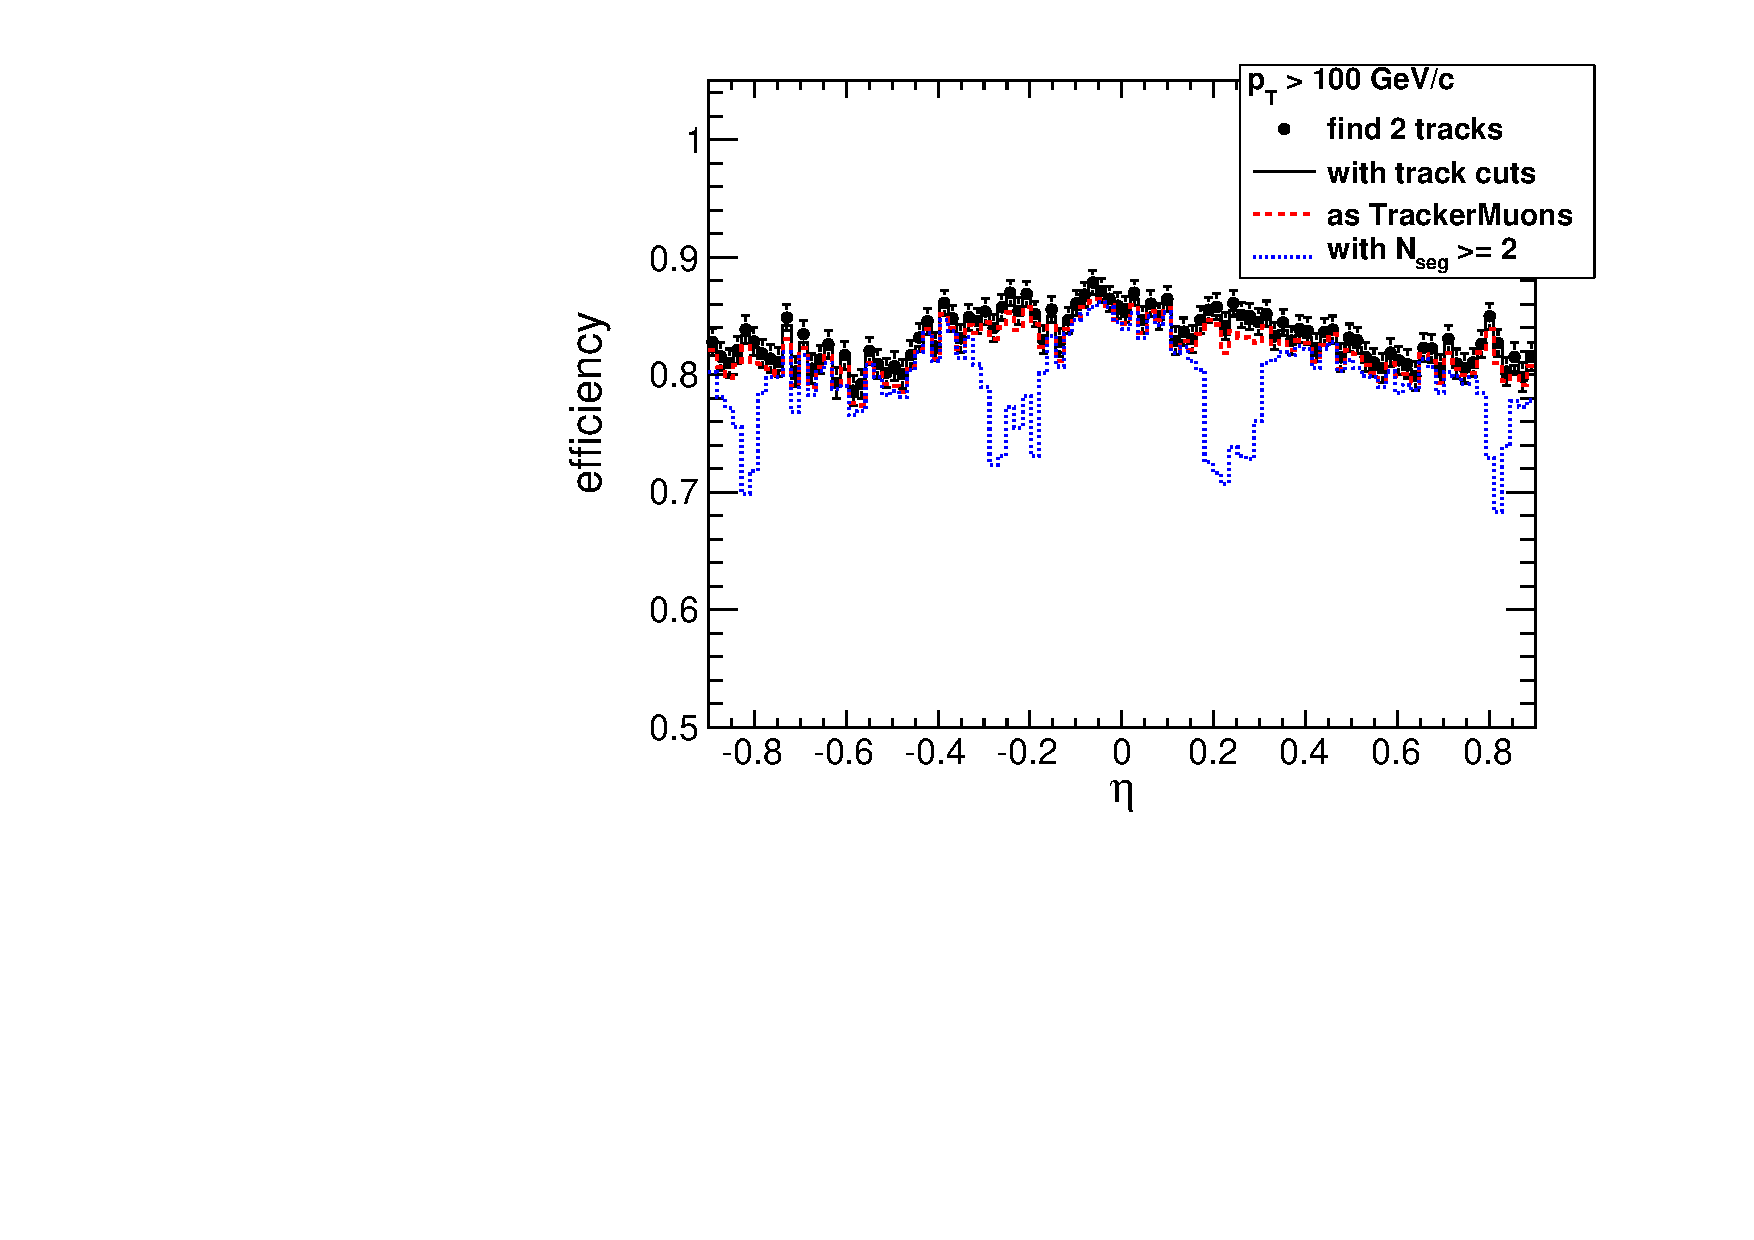
\includegraphics[width=0.48\linewidth]{PLOTS/HIGHPT_STUDY/highptstudy_eta.pdf} \hfill
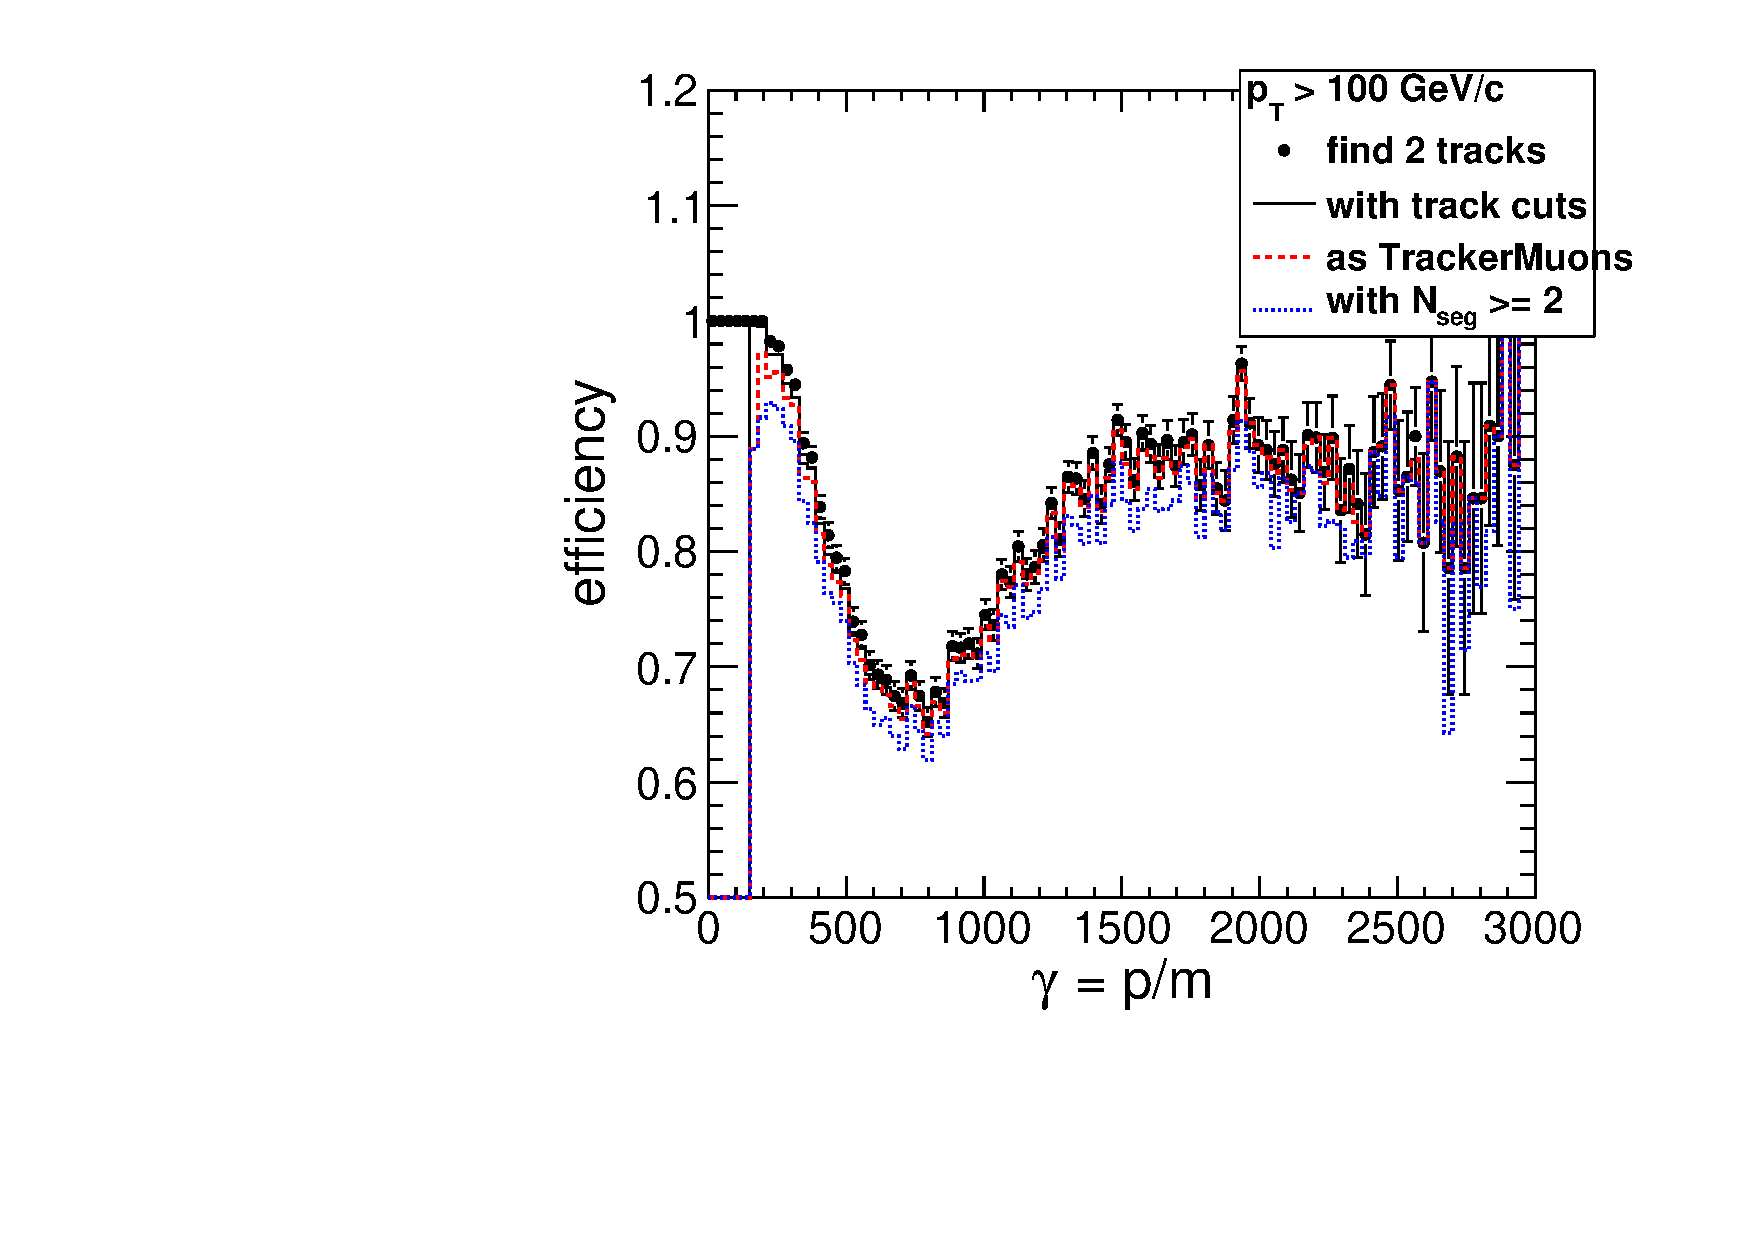
\includegraphics[width=0.48\linewidth]{PLOTS/HIGHPT_STUDY/highptstudy_gamma.pdf}
\end{center}
\caption{Probability of passing each of the four stages of cuts, given that two muons exist at generator
level as a function of muon pair $p_T$ (a), invariant mass $m(\mu\mu)$ (b), $\eta$ (c), and the relativistic boost $\gamma$(d).
All distributions were obtained using the dimuon gun with flat distribution in the invariant mass of the pairs from 0.210 to 0.6 GeV/c$^2$ 
and $p_T(\mu\mu)$ from 0 to 500 GeV/c. \label{fig:highpttrackingstudy_kinematics}}
\end{figure}

As it was mentioned already, the dominant factor in the efficiency is the extent to which the two tracks overlap (and share hits) within 
the tracker volume. While this is a purely geometric effect, small systematic differences between the simulation predictions and the data if the 
sizes of the track hits (clusters) in the tracker could lead to a systematic deviation in the tracking efficiency in simulation. The proper
procedure to evaluate this effect, while technically complicated, would be to modify the size of the hits in tracker simulation by $\pm20$\% (a very
conservative figure) and re-measure the efficiency. A more simple, but nearly identical approach is instead of increasing
the size of the hits to ``push'' the two trajectories closer by the same 20\% and remeasure efficiency. Because the
distance between the tracks scales with $1/\gamma=m(\mu\mu)/p(\mu\mu)$, this can be accomplished by comparing the
efficiency for a given dimuon mass and $p_T(\mu\mu)$ points with efficiency at points with $p_T^{\prime}=(1\pm0.2)p_T(\mu \mu)$
and assigning the difference as the systematic uncertainty in tracking efficiency. Figures~\ref{tracking_eff_syst_estimation}(a),(b), and (c) 
show the efficiency of finding a dimuon pair (it also includes effects related to muon system in addition to tracking effect, but that inefficiency is
nearly independent of momentum) for $m(\mu\mu)=0.25$, 0.5 and 1 GeV/c$^2$. It also demonstrates the procedure for estimating the 
systematics uncertainty by shifting the efficiency curve by $\pm20$\% in muon pair $p_T$ to account for possible deviations in track cluster
sizes in the tracker simulation. Efficiency for $m(\mu\mu)>1$ GeV/c$^2$ is similar to what it is for $m(\mu\mu)=1$ GeV/c$^2$.

\begin{figure}
\begin{center}
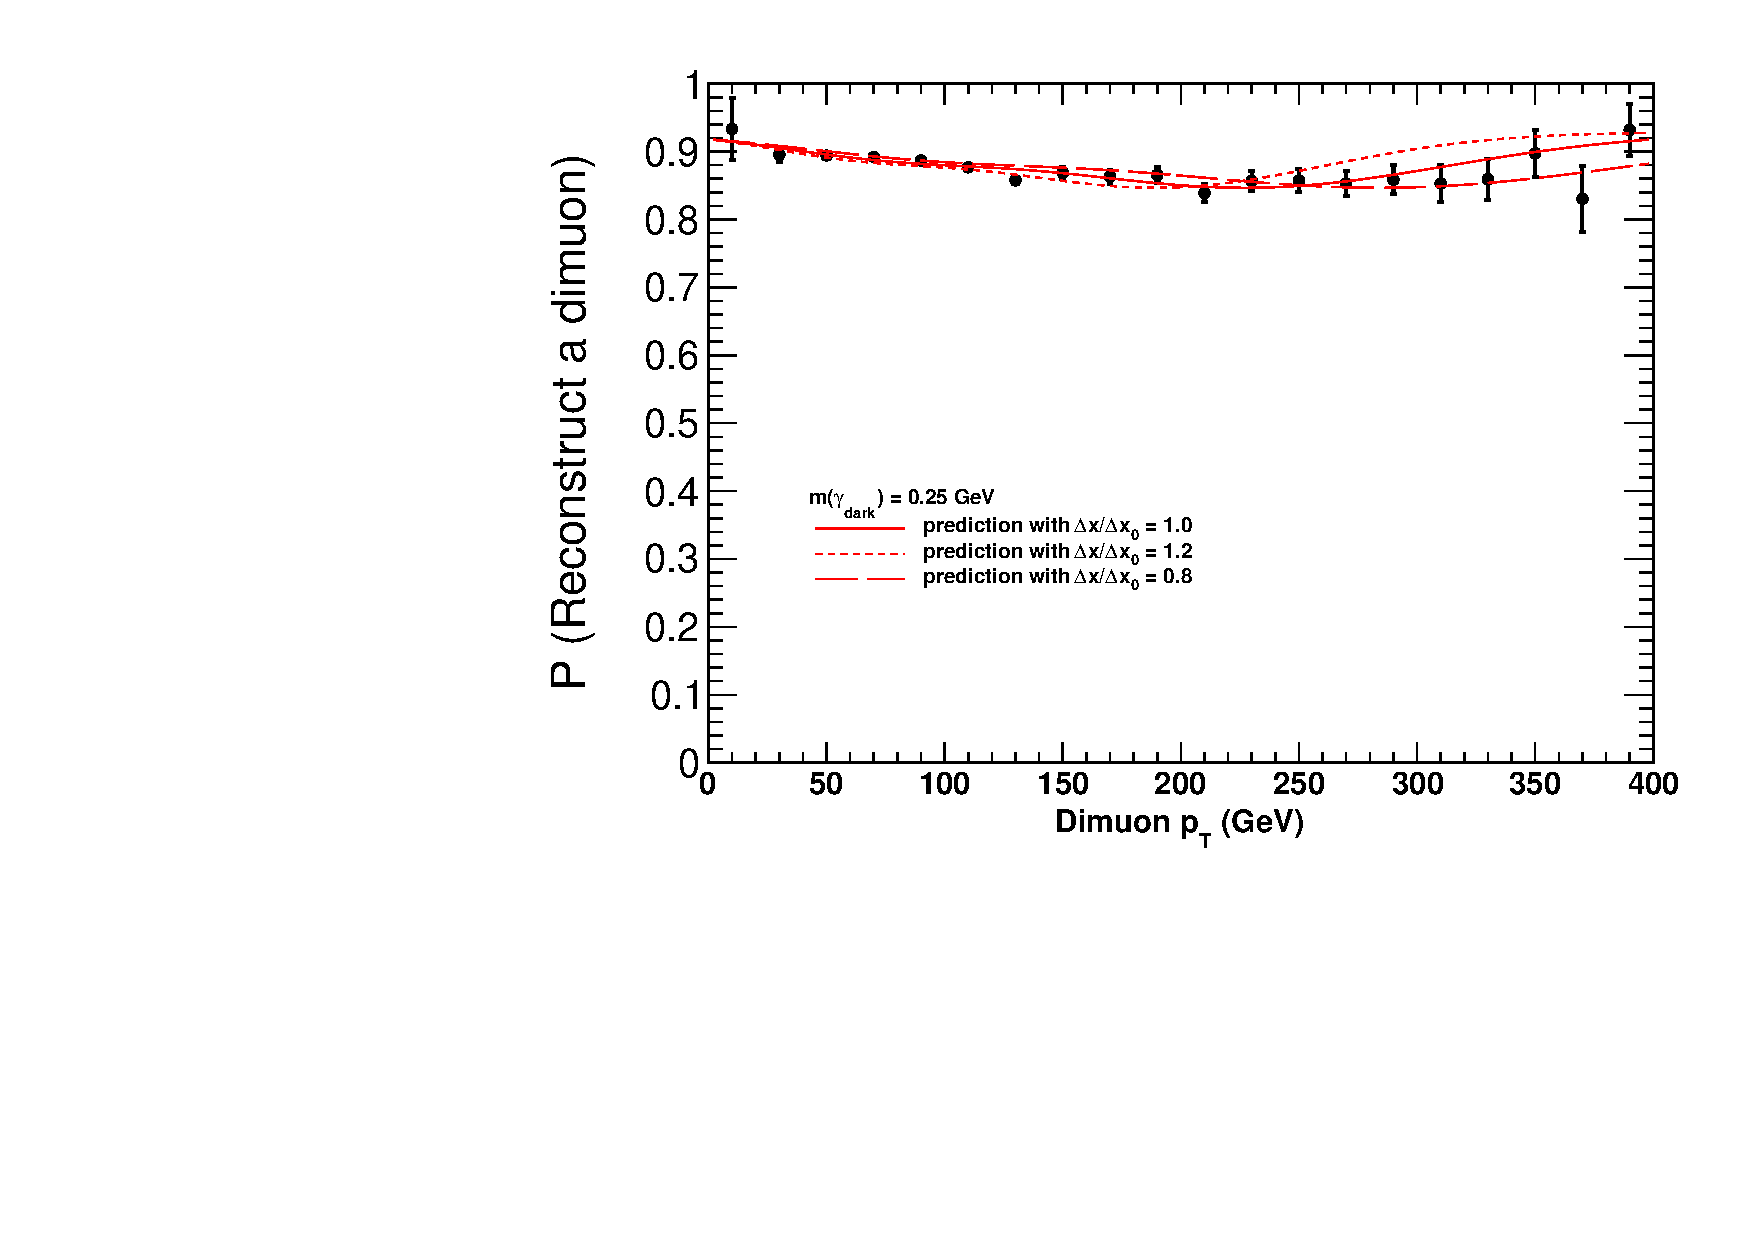
\includegraphics[width=0.32\linewidth]{PLOTS/appendix_p/025_03.pdf}
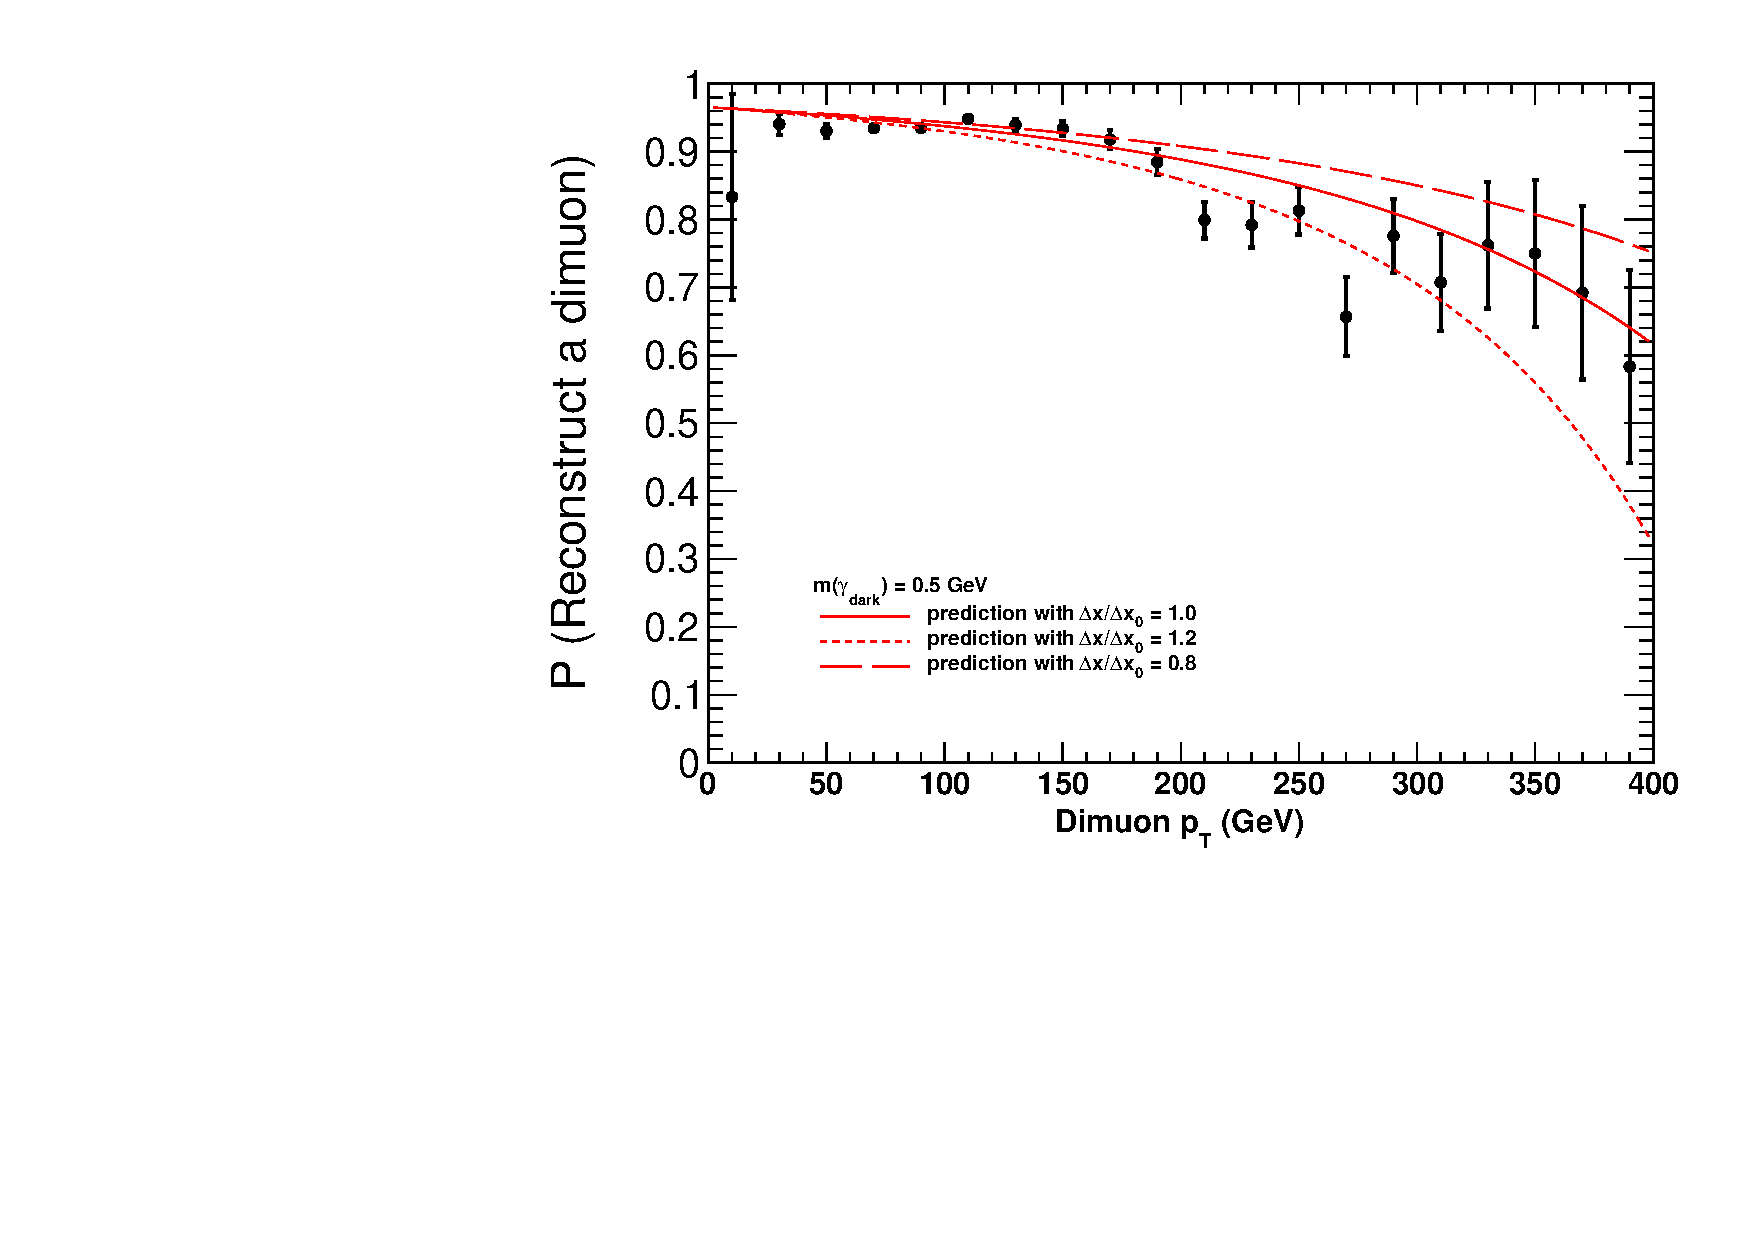
\includegraphics[width=0.32\linewidth]{PLOTS/appendix_p/050_03.pdf}
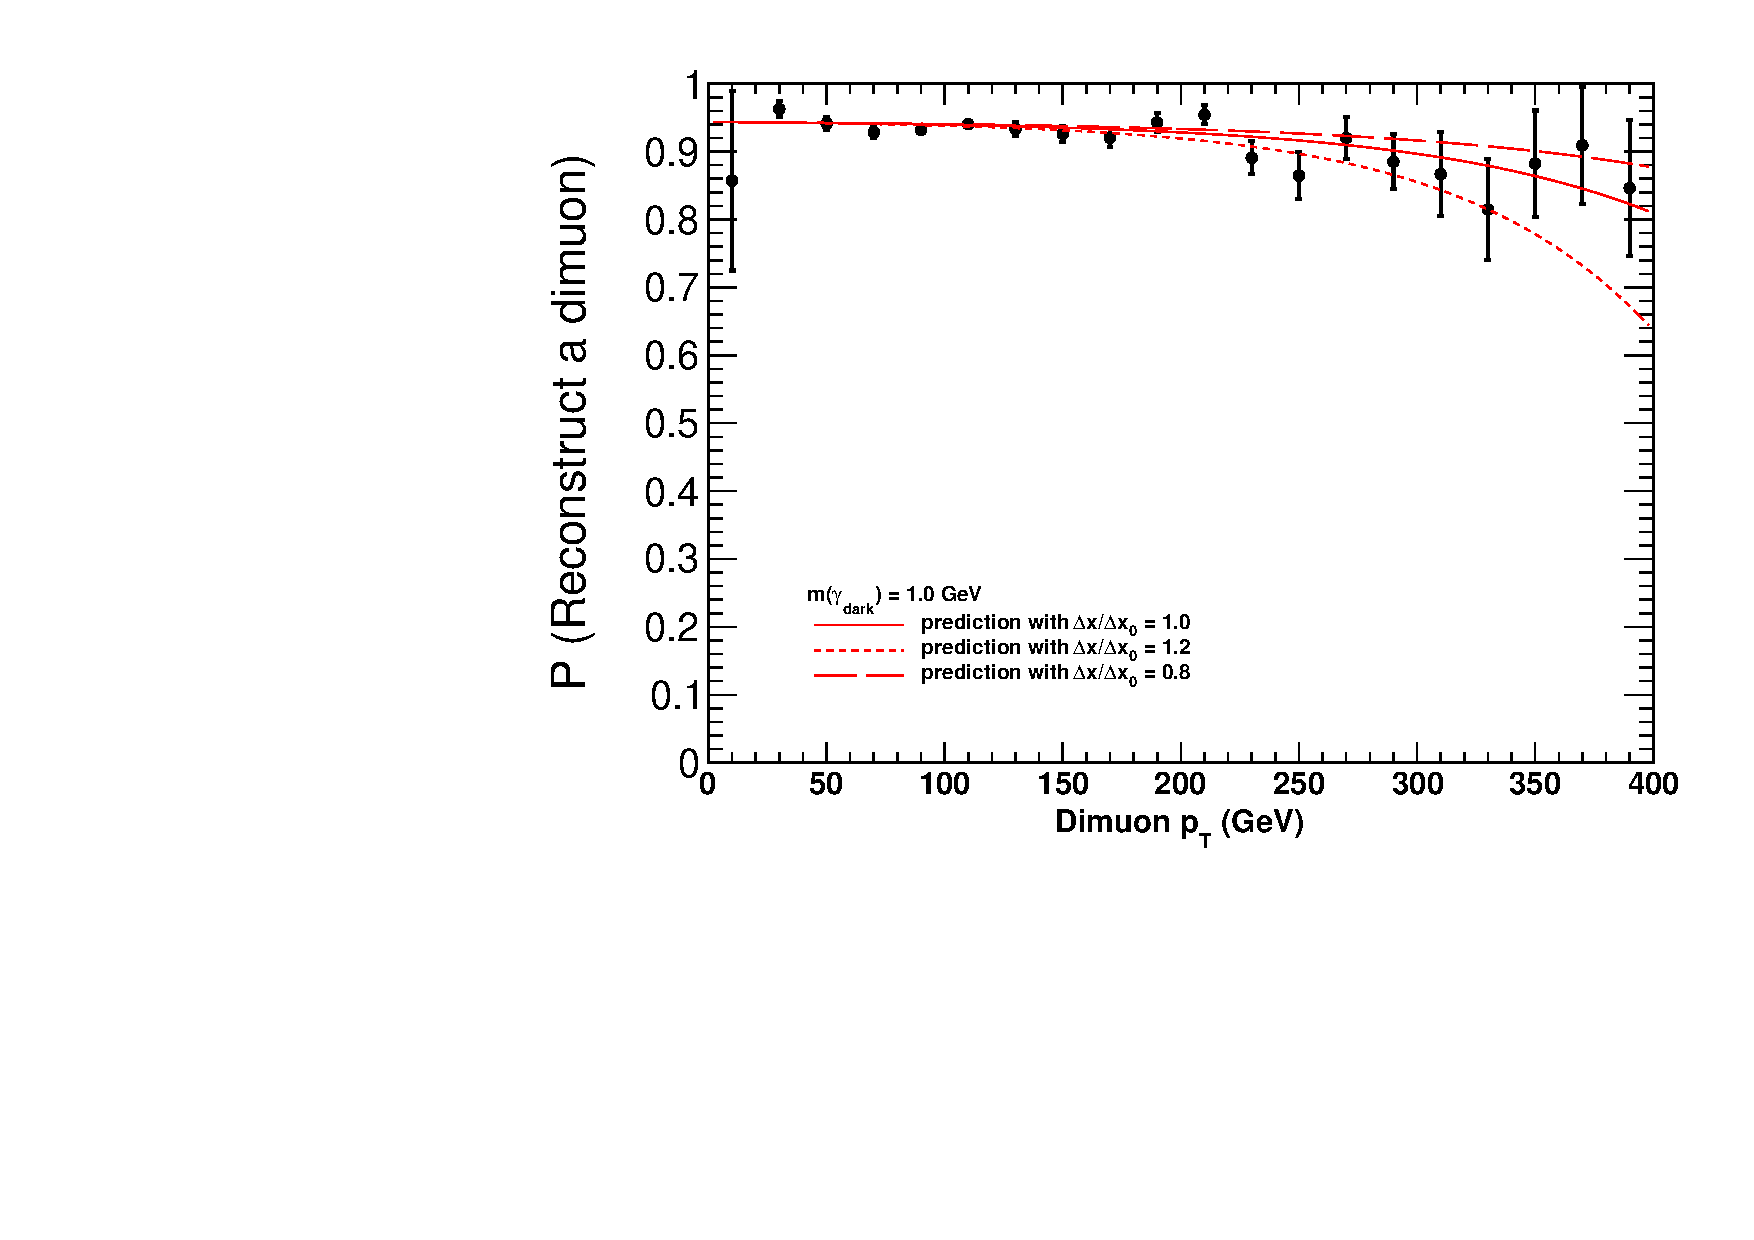
\includegraphics[width=0.32\linewidth]{PLOTS/appendix_p/100_03.pdf}
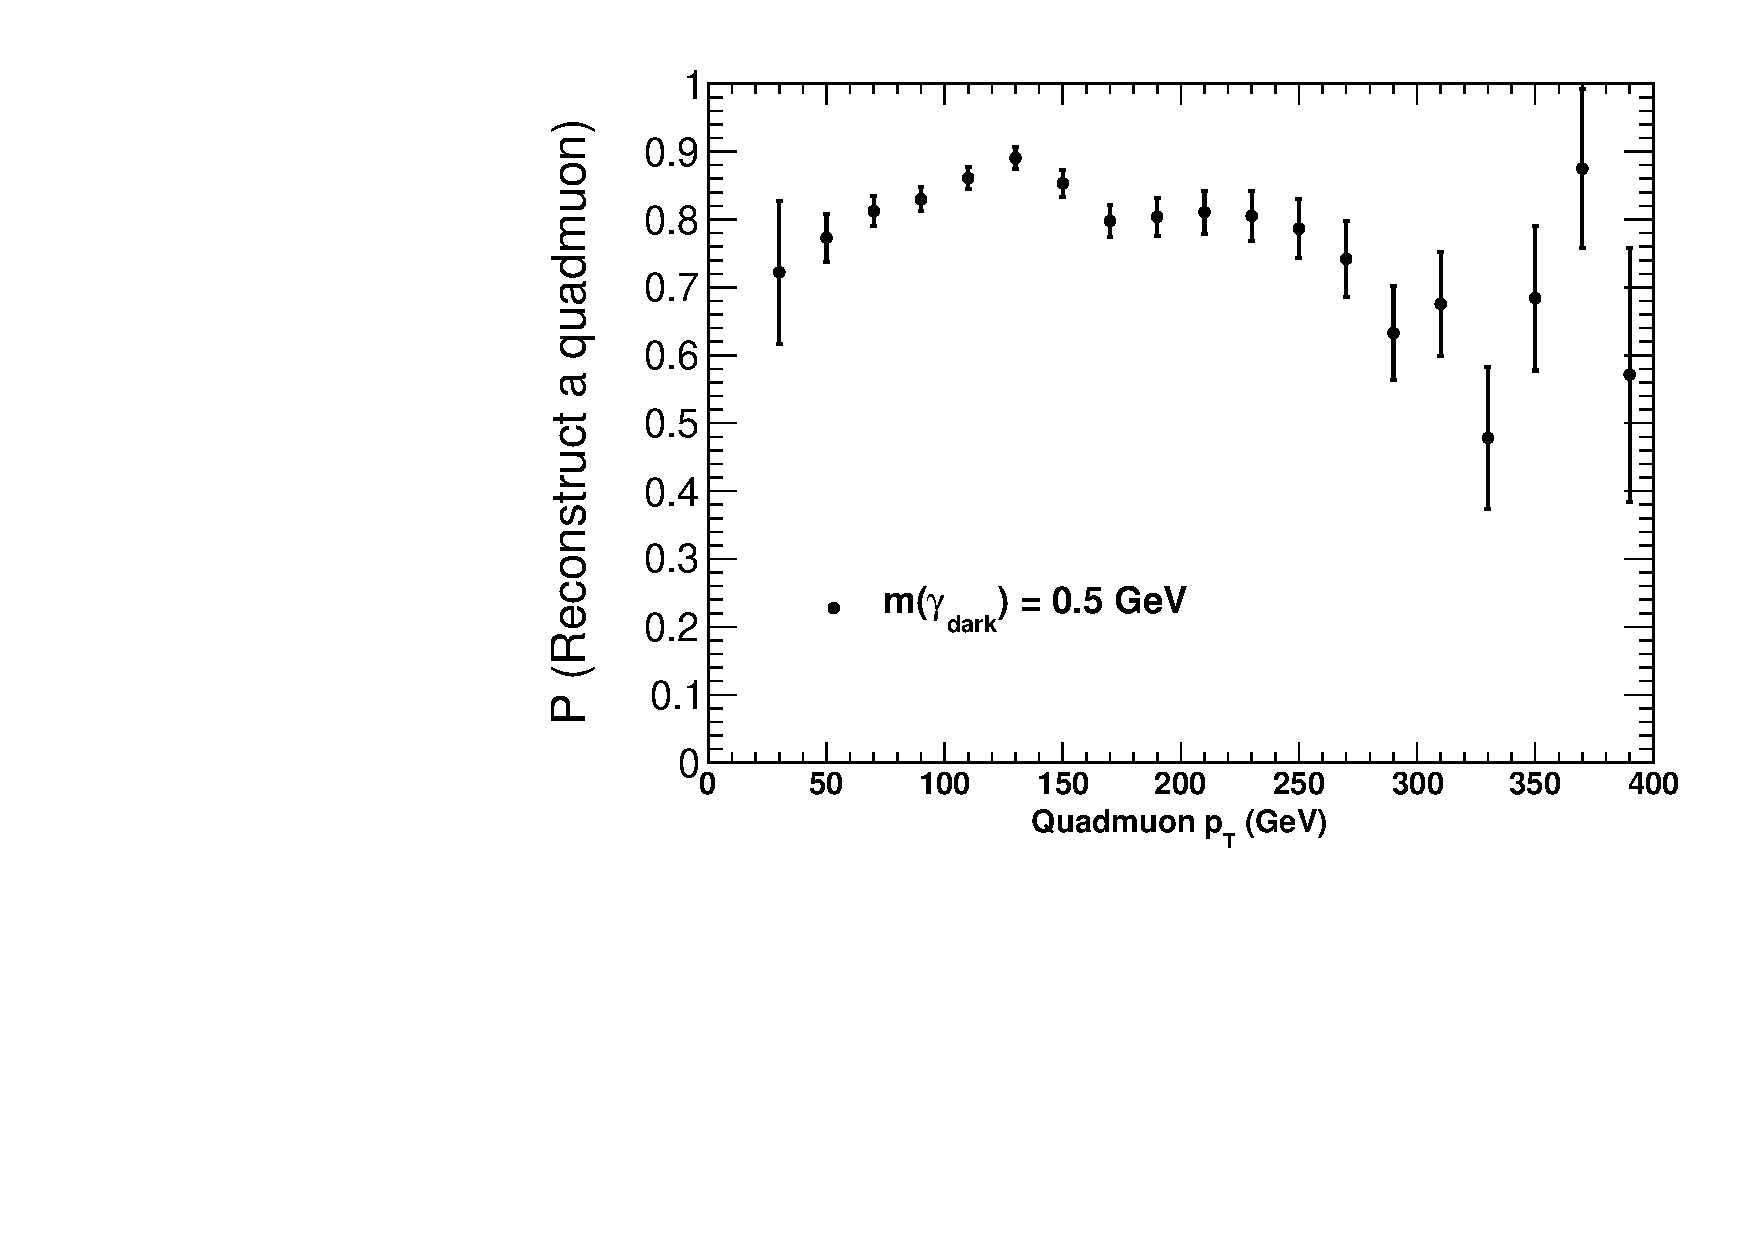
\includegraphics[width=0.32\linewidth]{PLOTS/appendix_p/01_eff_4mu_05.pdf}
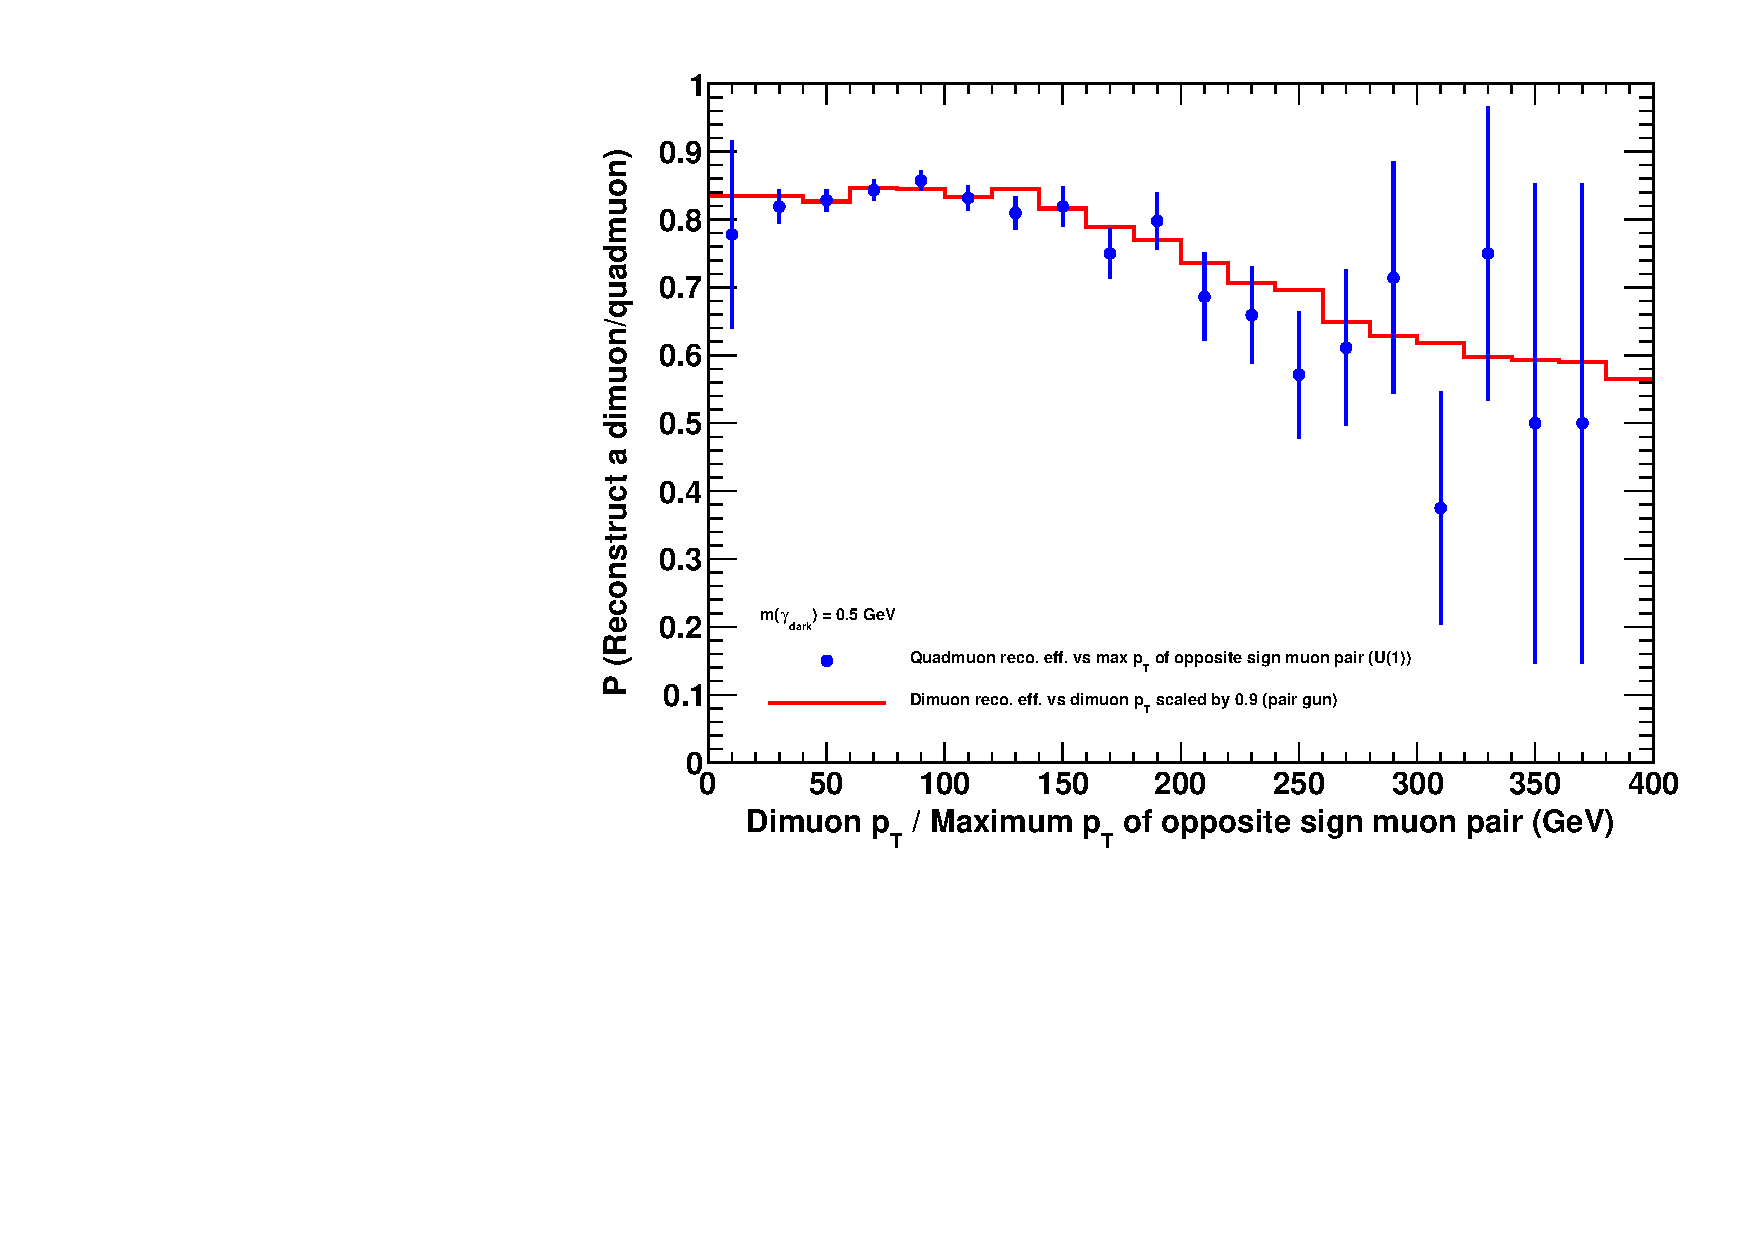
\includegraphics[width=0.32\linewidth]{PLOTS/appendix_p/04_eff_4mu_2mu_scaled.pdf}
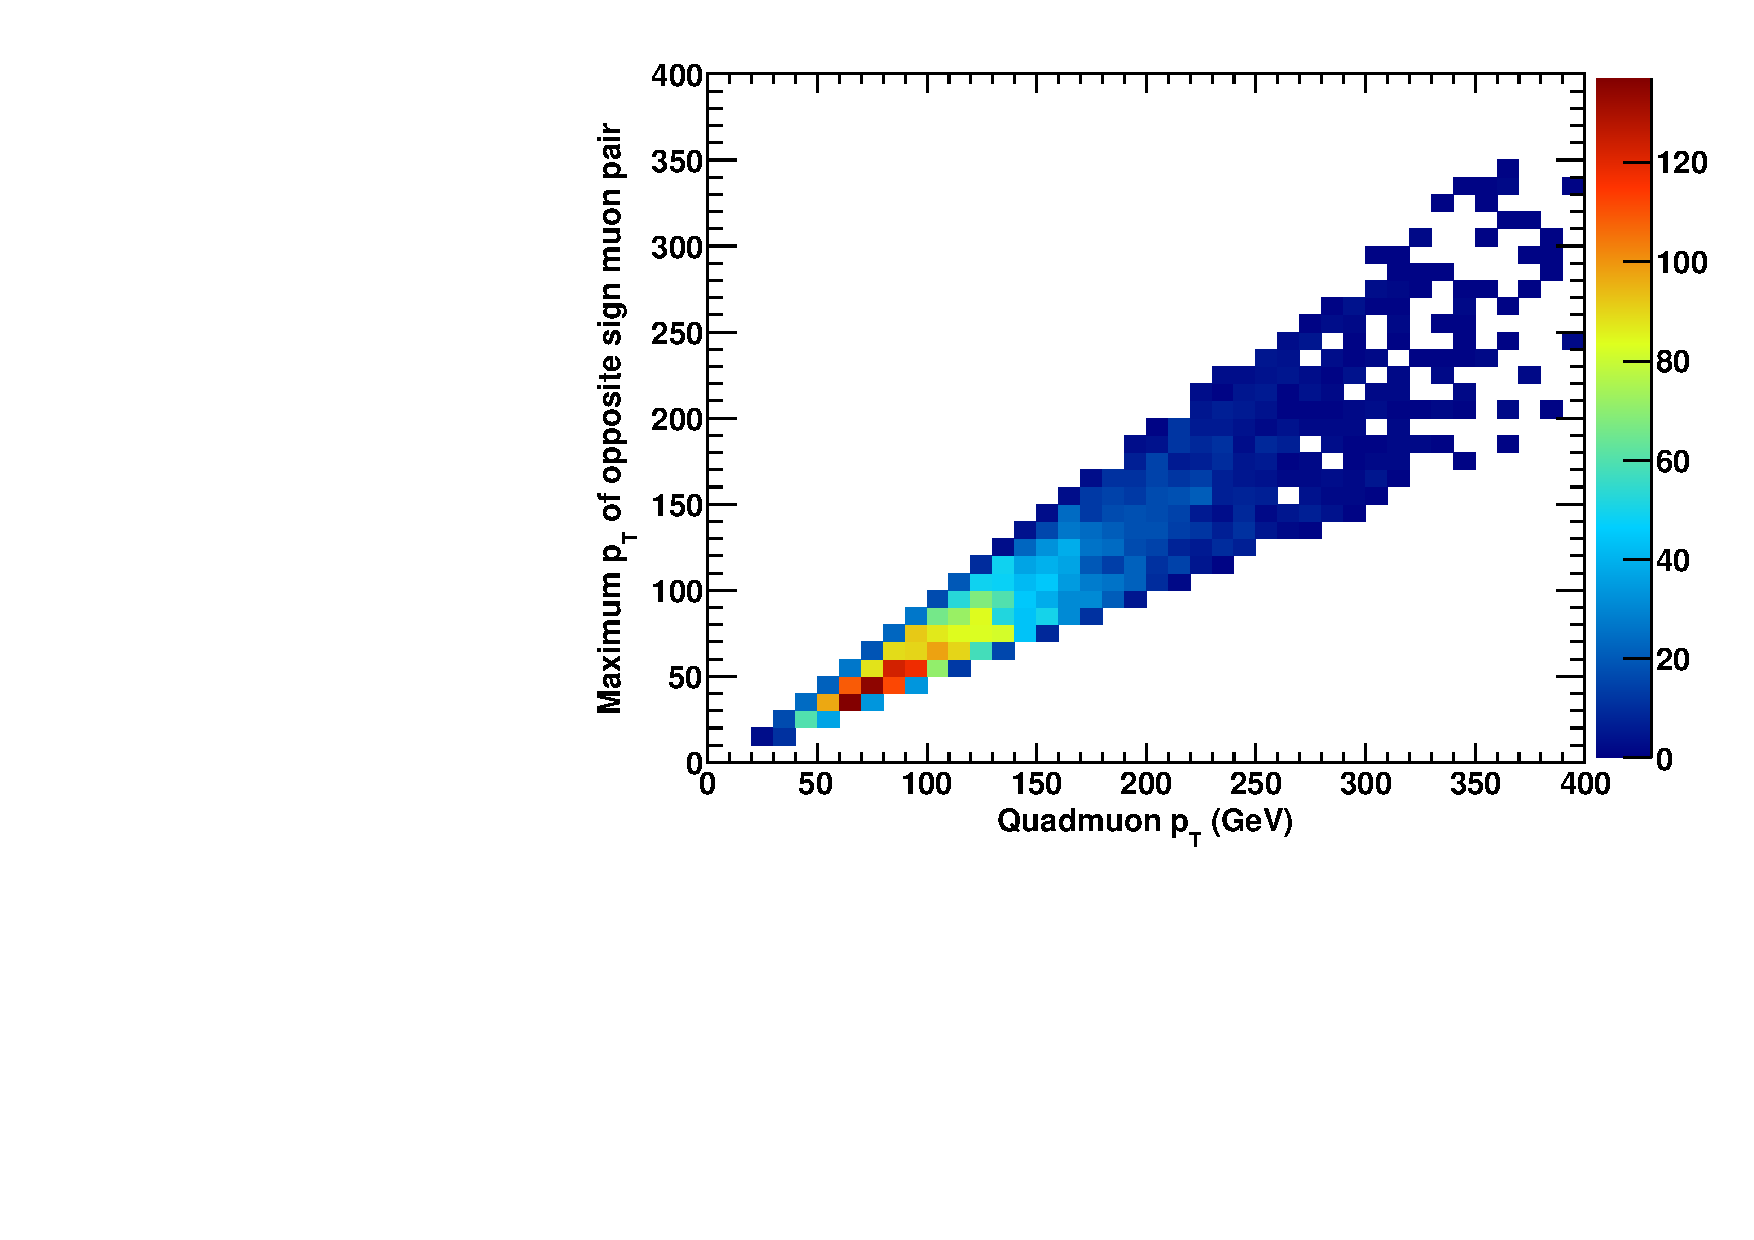
\includegraphics[width=0.32\linewidth]{PLOTS/appendix_p/02_4mu_pt_2mu_pt.pdf}
\end{center}
\caption{(a,b,c): Illustration of estimating the systematic uncertainty in tracking efficiency by fitting the efficiency of findinga  dimuon pair to a 
smooth curve $\epsilon(p_T)$ and using curves $\epsilon^{\prime}(p_T)=eps((1\pm0.2)p_T)$ to estimate the systematic uncertainty in tracking efficiency. 
Varying $p_T$ within 20\% approximately corresponds to varying the hit (cluster) size in tracker simulation by 20\%. Fits are performed separately for 
``cowboy'' and ``sailor'' toplogies and then combined in the plots for $m(\mu\mu)=0.25$ (a), 0.5 (b), and 1.0 GeV/c$^2$ (c). (d): Efficiency of finding 
a ``quadmuon'' from $h_d \to \gamma_d \gamma_d \to \mu\mu\mu\mu$ as a function of $p_T(\mu\mu\mu\mu)$, (e): the same efficiency plotted as a 
function of $p_T^{max}(\mu\mu)$ of the higher momentum muon pair overlaid with the efficiency of a singlle dimuon scaled to match the quadmuon
efficiency at lower $p_T(\mu\mu)$ showing that the tracking part of quadmuon efficiency finding is driven by the track finding efficiency of the higher
momentum pair, (f): distribution of $p_T^{max}$ of the higher momentum pair in a quadmuon versus quadmuon $p_T(\mu\mu\mu\mu)$ showing that
on average $p_T^{max}\sim 2/3 p_T(\mu\mu\mu\mu)$. \label{tracking_eff_syst_estimation}}
\end{figure}

For the models of interest, the efficiency of finding each muon pair in a higher multiplicity muon jet is nearly independent of other pairs because
the closest tracks are always those originating from the lowest mass dimuon resonance. Accidental substantial overlaps of the trajectories of 
muons from different nearby resonances are rare and do not dominate the uncertainty. In particular, the efficiency of reconstructing a ``quadmuon''
(shown in Fig.~\ref{tracking_eff_syst_estimation}(d)) is essentially a product of reconstruction efficiencies of the two dimuons within the quadmuon 
and is dominated by the probability to reconstruct the higher momentum pair. This observation is illustrated in Fig.~\ref{tracking_eff_syst_estimation}(e)
showing the quadmuon efficiency plotted as a function of the higher momentum dimuon within the quadmuon overlaid with the reconstruction efficiency 
of a single dimuon of the same momentum (the latter is scaled to agree with the quadmuon efficiency at low $p_T$ to remove the offset due to 
the efficiencies related to reconstructing the muons in the second pair in the muon system). Finally, Fig.~\ref{tracking_eff_syst_estimation} shows
the transverse momentum of the more energetic dimuon within the quadmuon versus transverse momentum of the quadmuon. One can conclude 
that $p_T^{max}(\mu \mu) \sim p_T{\mu \mu\mu\mu}$ allowing a simple translation of the tracking related part of the dimuon reconstruction efficiency 
and systematics into the reconstruction efficiency and systematics for the quadmuon. The same logic applies to higher multiplicity muon jets, but
note that kinematically accessible higher multiplicity muon jets will have on average lower momentum of constituent dimuons leading generally to higher 
overall reconstruction efficiency. This is because the same energy is essentially divided between higher number of dimuons. We also re-iterate our 
conclusion that the reconstruction efficiency for dimuons in events with nearby track pairs (e.g. in $h_d \to \gamma_d \gamma_d \to \mu^+ \mu^-  e^+e^-$) is essentially the same as for standalone dimuons.

Summarizing, we assign a systematic uncertainty due to tracking using plots in Fig.~\ref{tracking_eff_syst_estimation}. For reference, for $p_T=150$ GeV/c,
the systematic uncertainty for dimuon reconstruction efficiency due to tracking is 2,5, and 2\% for $m(\mu\mu)=0.25$, 0.5 and 1.0 GeV/c$^2$, respectively.
For quadmuons of $p_T=150$ GeV/c, the tracking uncertainty is under 2\% independent of mass and is approximately corresponds to dimuon efficiency 
at $p_T=100$ GeV/c ($2/3$ of th quadmuon $p_T$). For higher multiplicity lepton jets, the uncertainty is taken from the quadmuon case, which is a 
conservative estimate. These figures are used to estimate the efficiency for more complex event topologies with multiple muon jets, in which case the
uncertainties for each lepton jet are taken to be 100\% correlated.

\subsection{Trigger Selections}
\label{sec:trig_selections}
Trigger choice is an important consideration for this analysis because
the presence of nearby muon hits can potentially affect trigger
performance. Indeed, it was found that the trigger is substantially
inefficient for muons whose trajectories cross in the muon endcap,
though not the barrel.  The non-isolated, single-muon trigger response
is studied in the same way as
Sec.~\ref{sec:reconstruction_and_efficiency}, and presented in
Fig.~\ref{fig:triggerefficiency}(a).  See
Appendix~\ref{sec:motivation_for_trigger_choice} for an explanation of
why we chose non-isolated and single-muon triggers only.  As described
in Sec.~\ref{sec:reconstruction_and_efficiency}, inefficiencies that
depend on whether the muon trajectories cross are undesirable in a
model-independent analysis.  For this reason and because of the many
changes in the Endcap Level 1 ghost cancellation parameters during the
data taking period, events were required to be triggered in the barrel
($|\eta| < 0.9$).  The lowest-threshold, unprescaled trigger also
changed from 9 to 15~GeV/$c$ during the data-taking period, so we
select events with the 15~GeV/$c$ when available and simulate it by
requiring a trigger candidate of at least 15~GeV/$c$ for data before
its introduction.

While the above selections ensure robust L1 trigger performance, the
correlated muon effects may potentially introduce inefficiencies at
the level of the High Level Trigger (HLT). Because muon reconstruction
in the HLT closely follows the global muon reconstruction used in the
offline, the trigger efficiency can potentially suffer from correlated
effects due to the presence of nearby muon segments. Such inefficiency
would have caused a substantial effect on this analysis should we
required two reconstructed trigger muon candidates, however we only
require one muon to be reconstructed, so the efficiency of finding the
higher $p_T$ muon remains high; see
Fig.~\ref{fig:triggerefficiency}(b).

Because the barrel muon trigger efficiency does not suffer from the
correlated effects observed in the endcap to any significant degree,
the trigger efficiency is calculated using simulation and corrected
with a uniform scale factor of $0.968 \pm 0.004$ per event is obtained
from $Z \to \mu\mu$ data and simulation using a tag-and-probe
technique (see Appendix~\ref{sec:tag_and_probe}).

\begin{figure}[tbh]
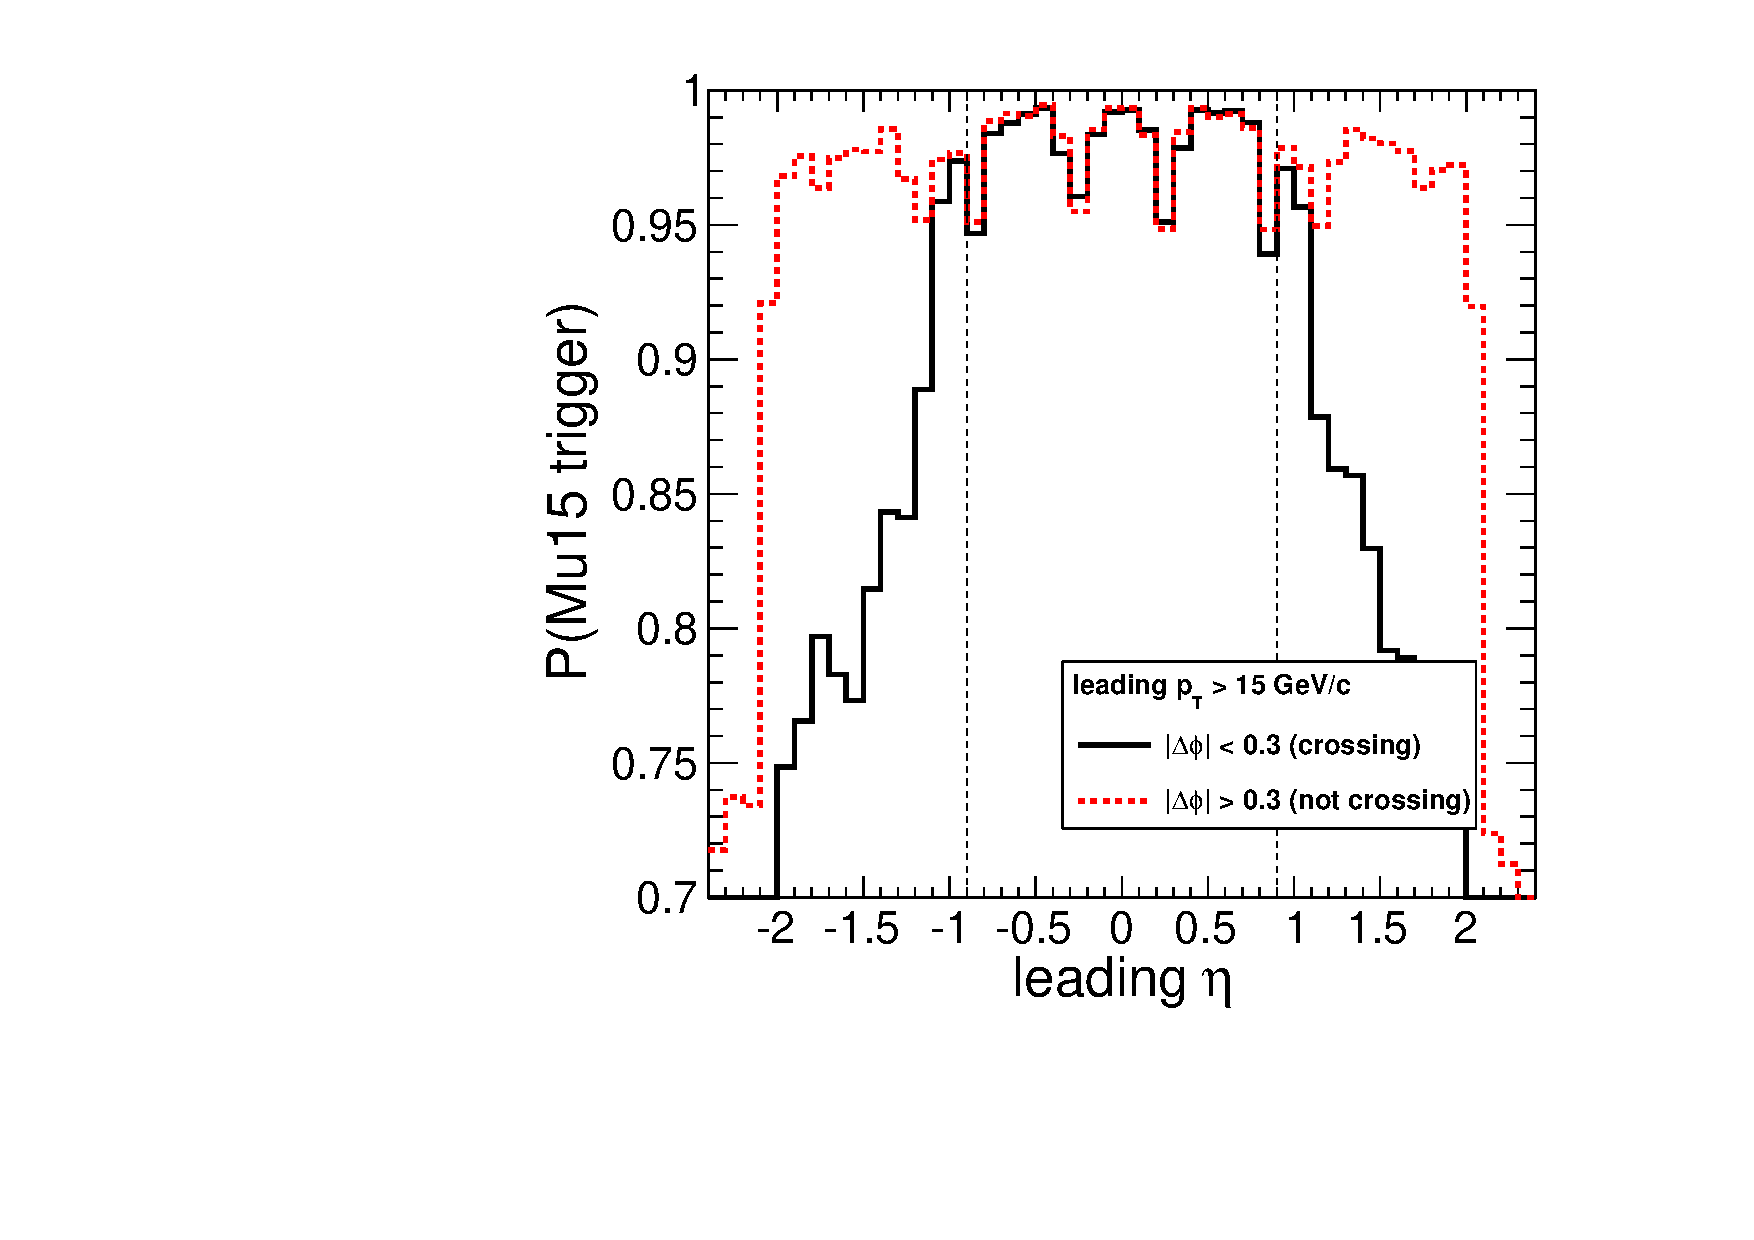
\includegraphics[width=0.48\linewidth]{PLOTS/eta_mass5cut_triggerMu15.pdf} \hfill
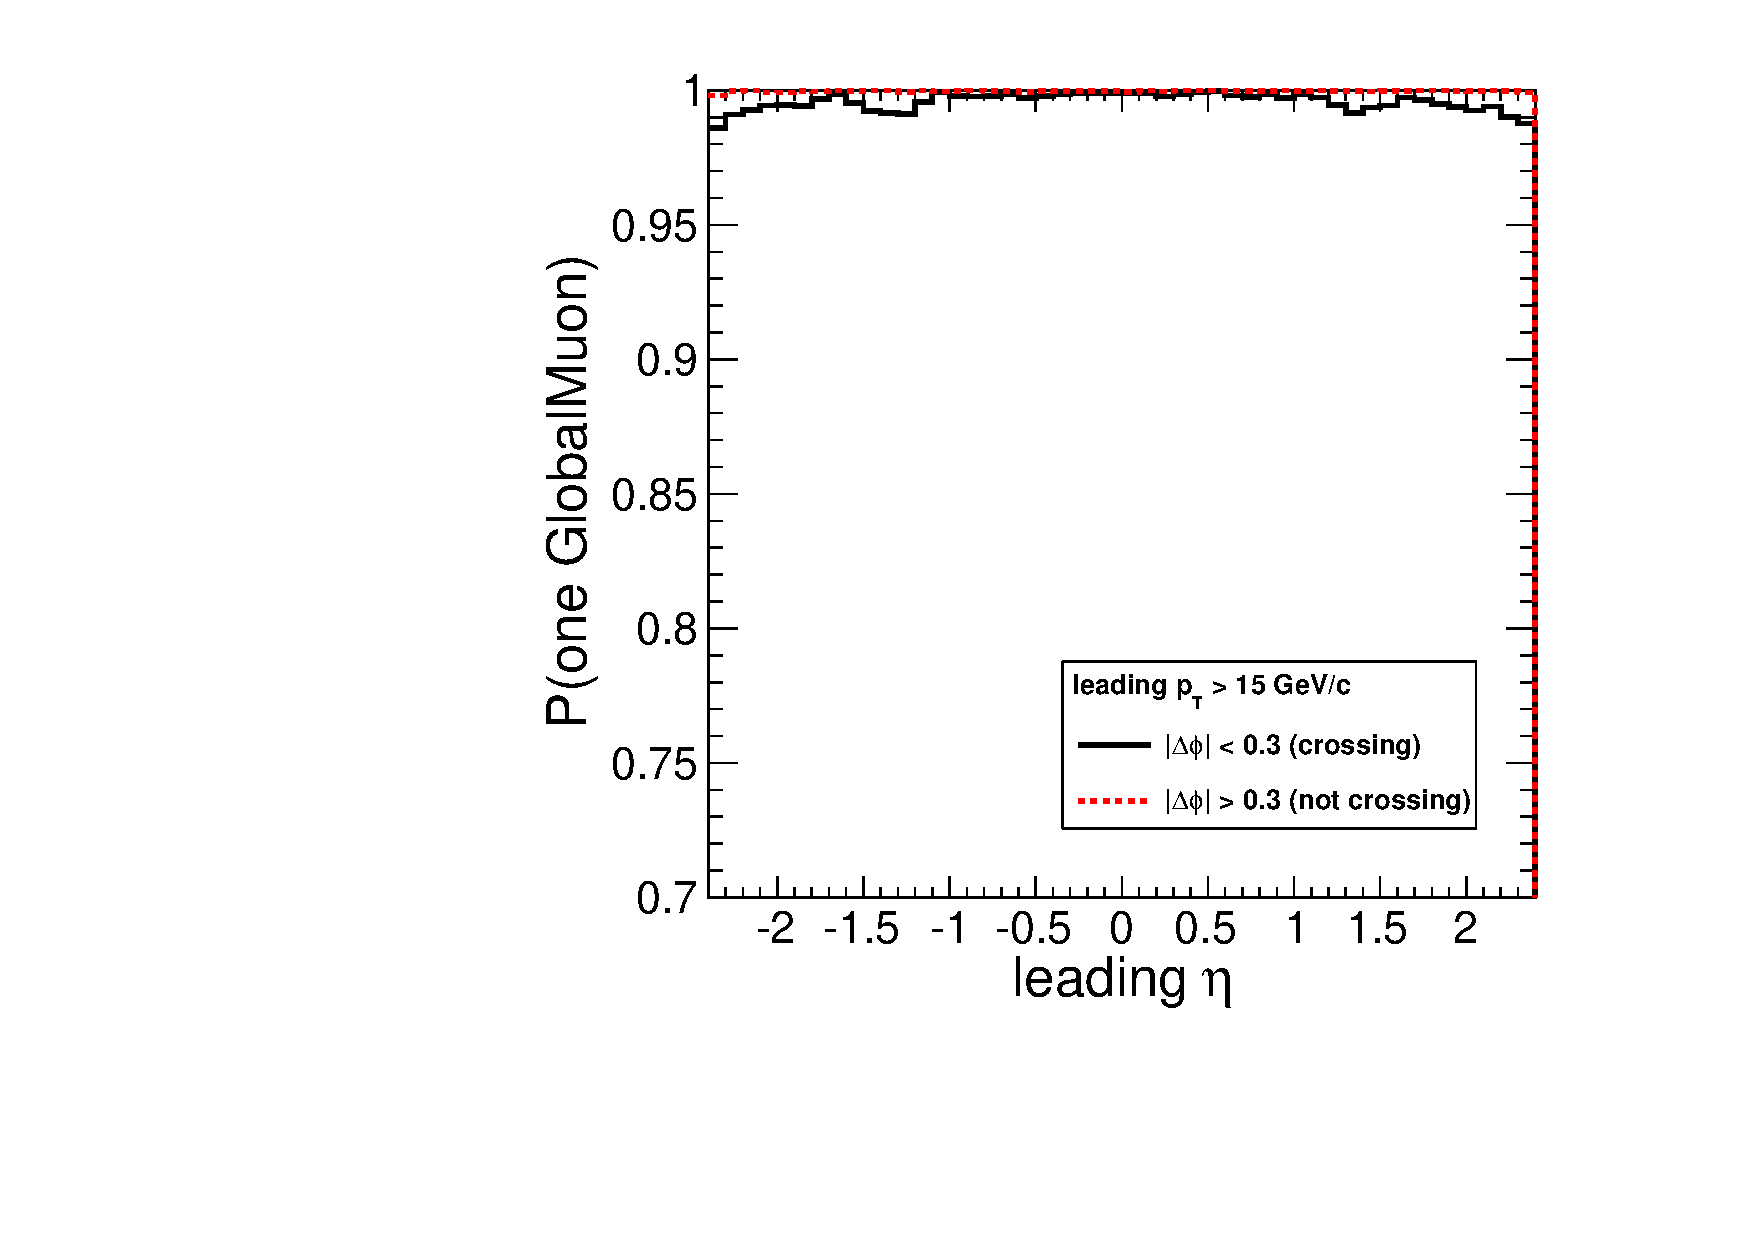
\includegraphics[width=0.48\linewidth]{PLOTS/eta_mass5cut_oneGlobalMuon.pdf}
\caption{Left: non-isolated, single-muon, $p_T > 15$~GeV/$c$ trigger
  efficiency (L1 and HLT).  Right: probability of finding one $p_T >
  15$~GeV/$c$ GlobalMuon (algorithm used by the HLT). \label{fig:triggerefficiency}}
\end{figure}

\subsection{Modeling of the Signal Dimuon Resonance Mass Spectrum}
\label{sec:signal_mass_spectrum_shape}

Because the new resonances decay to Standard Model particles only and the coupling to SM is weak, they have narrow width and the shape of the di-muon invariant mass distribution is fully determined by the detector resolution and final-state radiation of a photon from one of the muons. Though extreme precision in modeling these shapes is not required in the presence of nearly zero backgrounds, it has to be reasonably well-understood if we need to quantify properties of the new resonances, assuming they are discovered.

The Standard Model provides four narrow, high cross-section dimuon resonances in our mass range of interest, $\omega$, $\phi$, $J/\psi$, and $\psi'$, which we use to calibrate the signal lineshapes.  We study the resolution of each of these resonances in data using a suitably defined function (Crystal Ball with separate core resolutions for the barrel and the endcap) and find a good agreement with the expectation based on simulation predictions (see details in Appendix~\ref{sec:appendix_signal_shape_studies}). 

\begin{figure}[tbh]
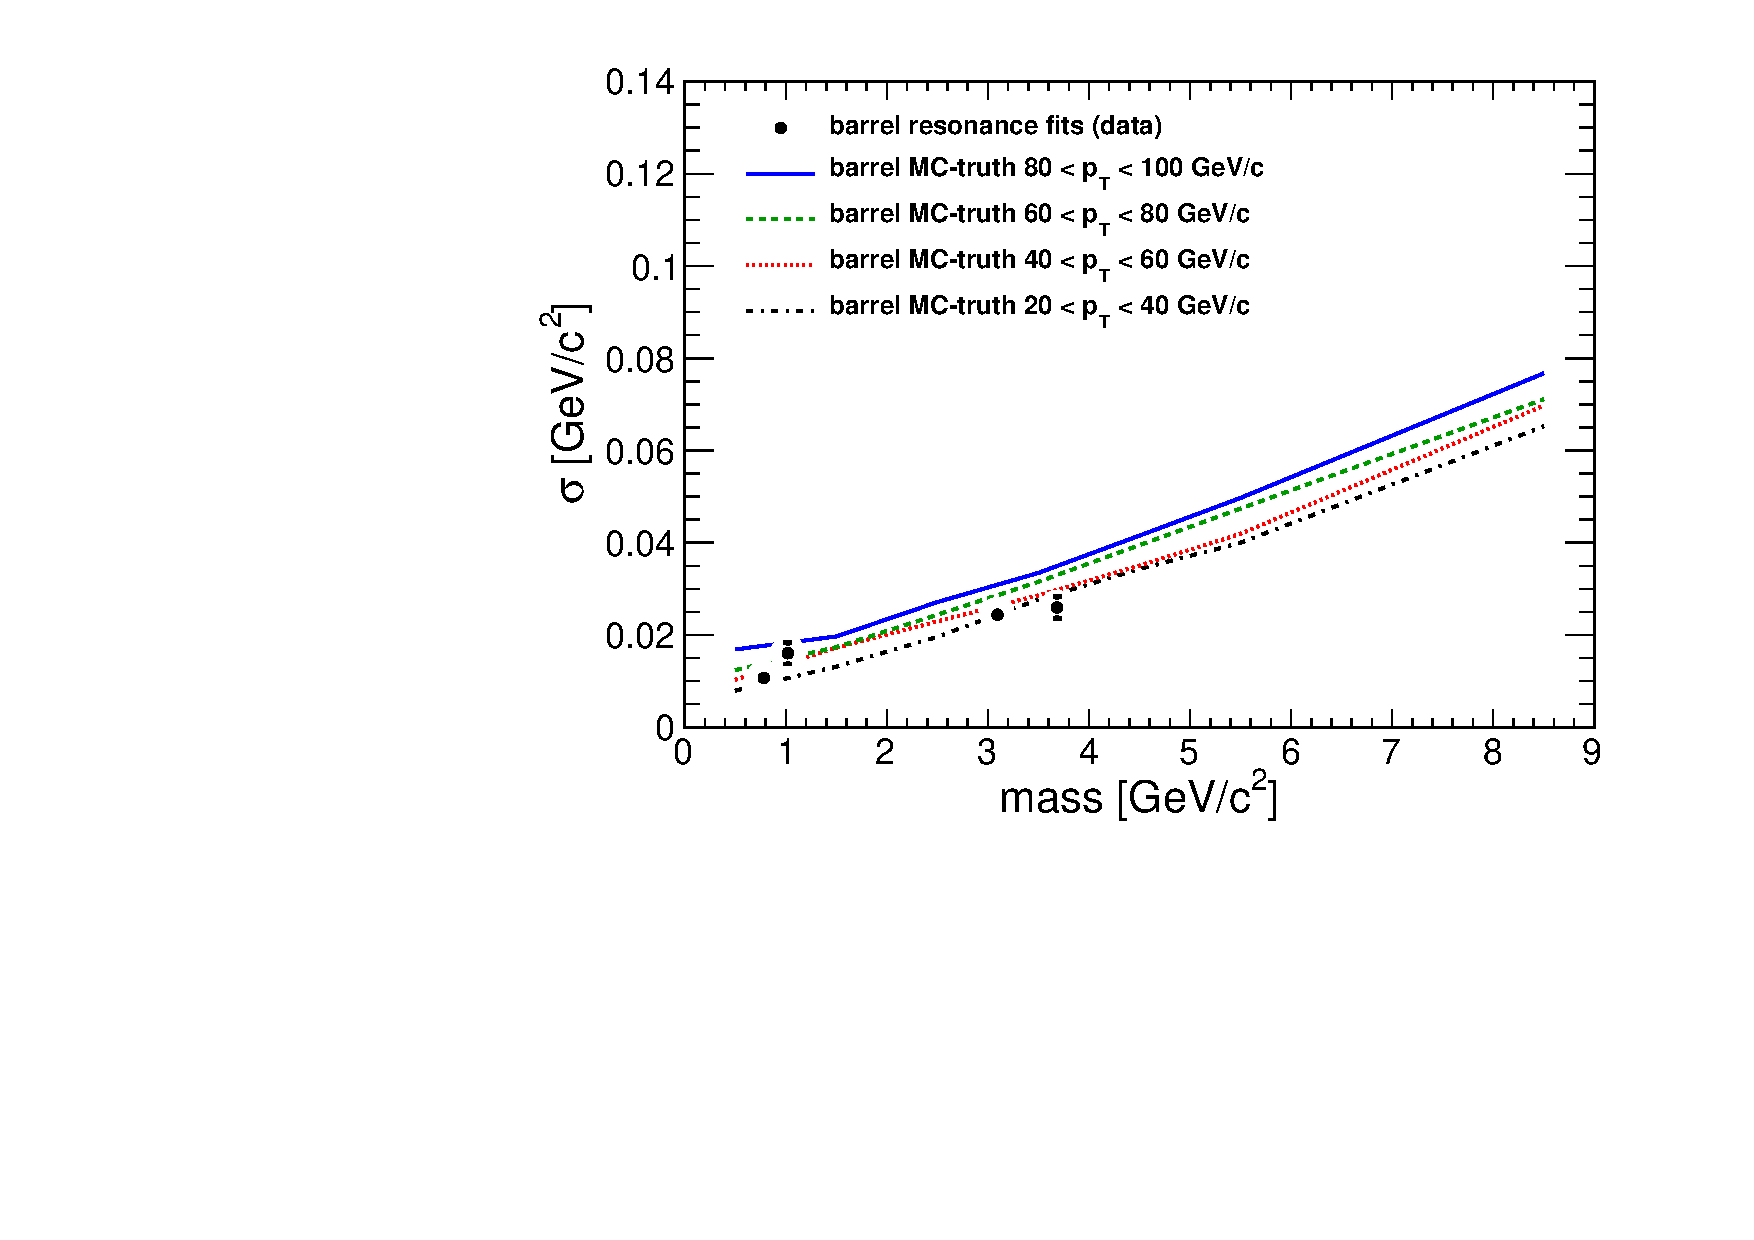
\includegraphics[width=0.5\linewidth]{PLOTS/resolution_barrel.pdf}
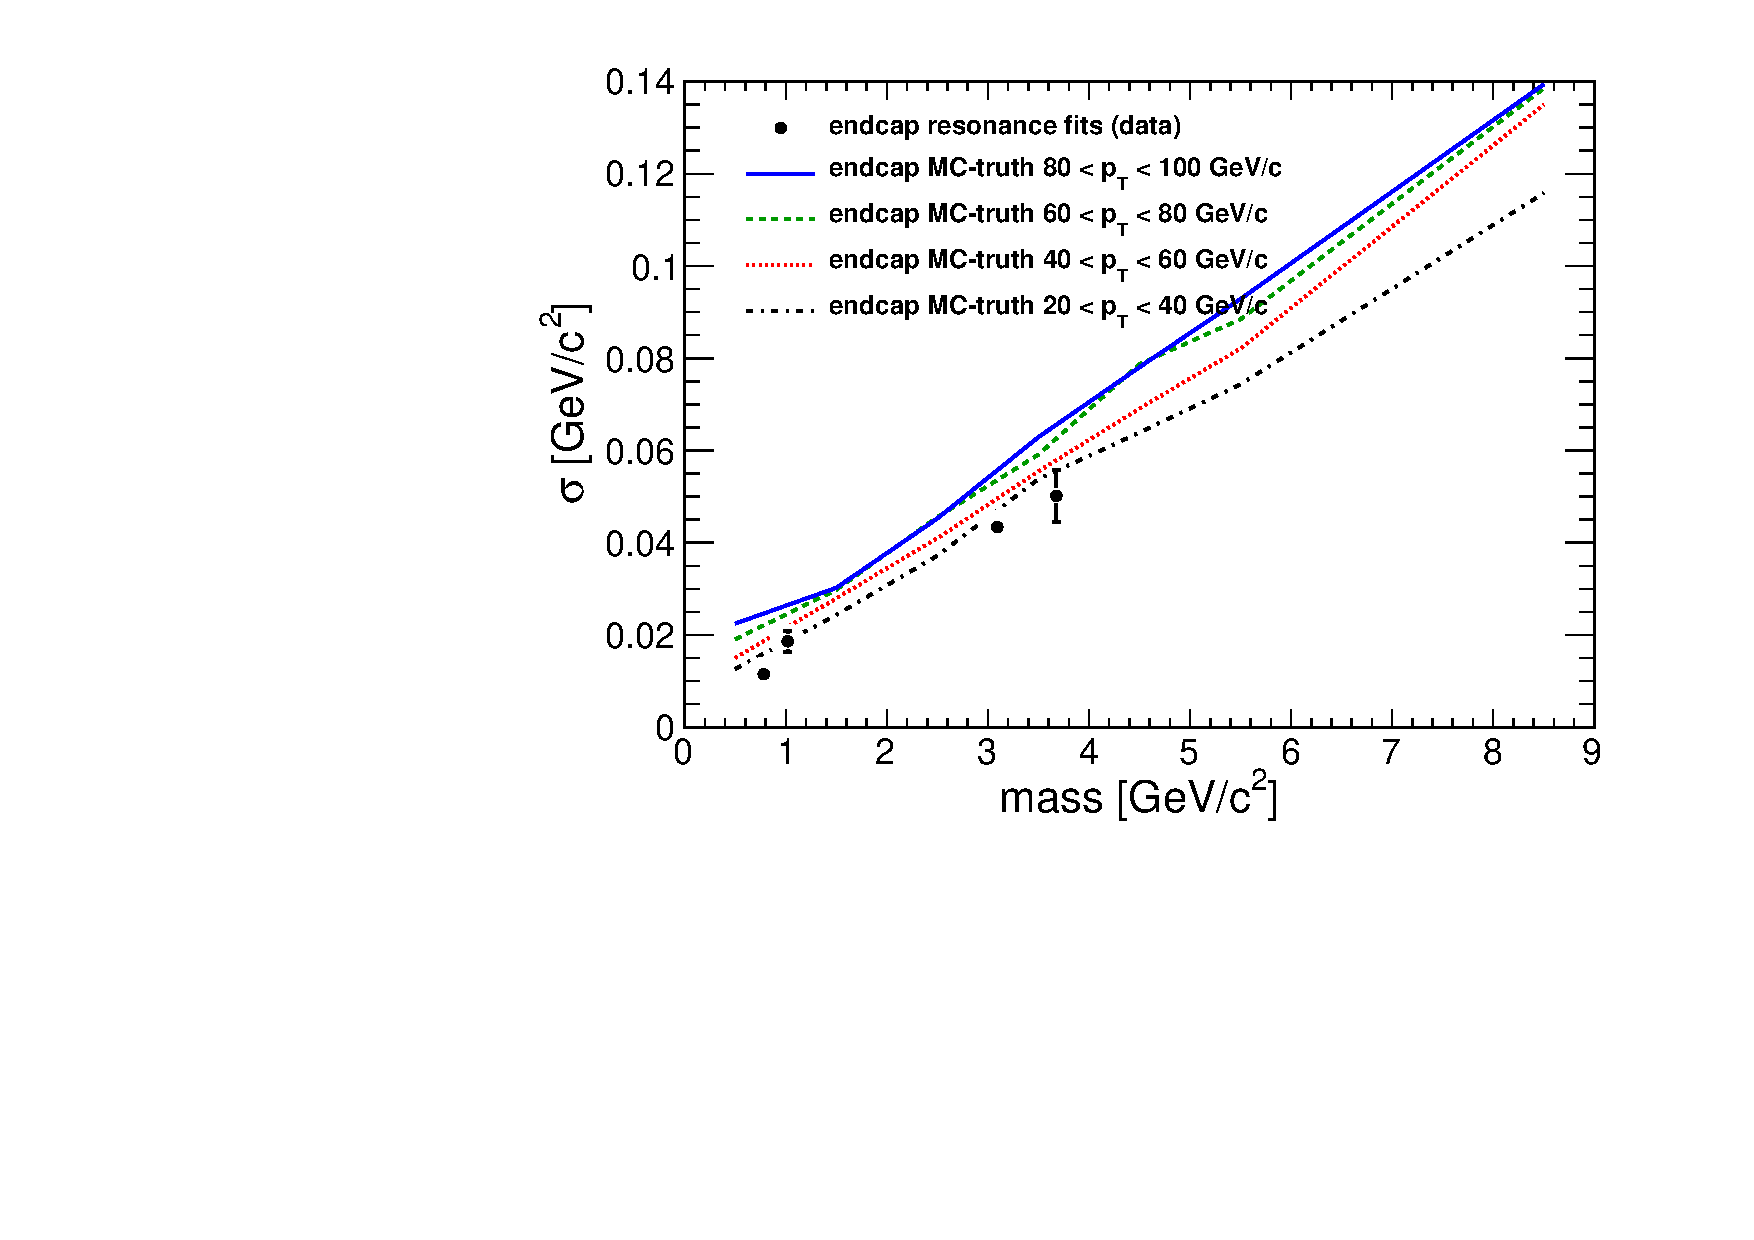
\includegraphics[width=0.5\linewidth]{PLOTS/resolution_endcap.pdf}
\caption{Left: resolution as a function of mass for simulated muons
(lines) and real resonances (points) in the barrel region $|\eta|<0.9$ as obtained using the fit to a Crystal Ball shape.  Right: the same distributions for the overlap and endcap region $|\eta|>0.9$. \label{fig:resolution}}
\end{figure}

To study the systematics effects, we note that the resolution of the low mass resonances depends on the mass of the resonance, momentum (boost) of the resonance and also have an $\eta$-dependent component associated with lower resolution in the forward region. Figure~\ref{fig:resolution}(a) shows the dependence of the core resolution on dimuon $p_T$ and resonance mass, overlaid with the results of the fits in data for regions with $|\eta|<0.9$ and $|\eta|>0.9$ (note that the momenta of resonances in data typically fall into the lowest  bin, $p_T$ = 20--30~GeV/$c$). Because the data and simulation agree well, we conservatively use the spread due to the dimuon $p_T$ shown in the figure as the systematic uncertainty for the core resolution parameter $\sigma$. The mean value used corresponds to the middle of the band and evolves with the mass of the resonance according to the dependency shown; the dimuon $p_T$ dependency is not included for simplicity. Note that while one of the muons in the distribution is typically a trigger muon, these resolutions are dominated by the tracker performance and are independent of the trigger: the trigger modifies the acceptance and efficiency, but this is not an issue for the shapes of the resonances.

We use these studies to define the signal regions in the multi-dimensional space of dimuon invariant masses as a ``corridor'' near the diagonal with the width of $5\sigma$ in detector resolution in each direction, where $\sigma(m,p_T) = 0.026 + 0.0065 m$ for the barrel and $\sigma(m,p_T) = 0.026 + 0.013 m$~GeV/$c^2$ for the endcap.

\subsection{Complete Acceptance, Event Categorization and Selection Efficiencies}
\label{sec:complete_acceptance}

To simplify interpretation of the model-independent results and allow for a comparison with specific theoretical models, we calculate acceptance and efficiencies at the generator level and the fully-reconstructed level for each signal region.  The acceptance is representative of geometric and kinematic cuts while the efficiency quantifies losses due to reconstruction and trigger effects. Acceptances predicted by simulation are corrected for systematic effects obtained from comparisons with data using approproiate scale factors and uncertainties and are propagated into the experimental reported acceptances. This is convenient because corrections for reconstruction and trigger efficiencies are much less dependent on the kinematics of the events and a comparison to different models can be obatined by recalculating acceptance at the generator level and adjusting the limit by the ratio of acceptances for a new model and one of our models.

Table~\ref{tab:acceptance_benchmarks} lists acceptances and efficiencies of the event selections and categorization into signal regions for several representative benchmark scenarios. The upper part of the table serves mostly as an illustration and shows cumulative efficiencies for applying the minimal acceptance (which is actually applied in this analysis) and shows how the acceptance would reduce if one were to require additional muons in the event (these selections were not applied). Each line in the upper part of the table shows the fraction of events satisfying given requirement and all previous requirements. The bottom part of the table shows actual reconstruction level acceptances for each of the topologies used in this analysis. These are defined relative to all signal events generated (i.e. they already include minimal acceptance). The overall acceptance for all topologies is therefore a sum of individual acceptances for each topology. Furthermore, because the regions are not overlapping, the sum of acceptances for each of the topologies with a given number of muons should be roughly equal to the efficiency of requiring the same number of muons in the uper part of the table. The difference is due to failures in reconstruction or, for the single dimuon region (a-1), is due to the additional kinematical requirement of a highly boosted dimuon $p_T>80$ GeV/c not applied in the uper part of the table.

\begin{table}[p]
\caption{Illustration of the acceptances and efficiencies of the event selections and categorization into signal regions for several representative benchmark scenarios. The upper part of the table serves mostly as an illustration and shows cumulative efficiencies for applying the minimal acceptance (which is actually applied in this analysis) and shows how the acceptance would reduce if one were to require additional muons in the event (these selections were not applied). Each line in the upper part of the table shows the fraction of events satisfying given requirement and all previous requirements. The bottom part of the table shows actual reconstruction level acceptances for each of the topologies used in this analysis. These are defined relative to all signal events generated (i.e. they already include minimal acceptance). The overall acceptance for all topologies is therefore a sum of individual acceptances for each topology. Furthermore, because the regions are not overlapping, the sum of acceptances for each of the topologies with a given number of muons should be roughly equal to the efficiency of requiring the same number of muons in the uper part of the table. The difference is due to failures in reconstruction or, for the single dimuon region (a-1), is due to the additional kinematical requirement of a highly boosted dimuon $p_T>80$ GeV/c not applied in the uper part of the table. Acceptances for regions (a-2) and (b-1) refer to the near-diagonal signal region only (within $5\sigma$ in detector resolution: $\sigma(m) = (0.026 + 0.0065\, b m)$~GeV/$c^2$, where $b=1$ for barrel and $b=2$ for endcap.).  \label{tab:acceptance_benchmarks}}
\begin{center}
\begin{tabular}{|l|c|c|c|c|}
\hline
Selections & NMSSM & U(1) & $n_2 (\to n_1 \gamma_{D})$ & $n_2 \to n_1 h_{D}(\to 2 \gamma_{D})$\\
\hline
 \multicolumn{5}{|l|}{Minimal Acceptance:} \\
\hline
$p_{T_1}>15$ GeV/c  &      &      &      &      \\
\& $|\eta_1| < 0.9$ & 58.0 & 88.2 & 77.2 & 81.0 \\ 
$p_{T_2}>5$ GeV/c   &      &      &      &      \\
\& $|\eta_2| < 2.4$ & 55.4 & 88.0 & 76.3 & 80.9 \\
\hline
\multicolumn{5}{|l|}{Additional Muons with $|\eta| < 2.4$:} \\
\hline
$p_{T_3}>5$ GeV/c   & 48.3 & 86.1 & 69.5 & 80.5 \\
$p_{T_4}>5$ GeV/c   & 26.9 & 78.6 & 48.5 & 78.4 \\
$p_{T_5}>5$ GeV/c   &  0.1 & 55.1 &  5.7 & 73.4 \\
$p_{T_6}>5$ GeV/c   &  0.0 & 35.1 &  0.6 & 63.4 \\
\hline \hline
\multicolumn{5}{|l|}{Categorization and Trigger} \\
\hline
(a-1) accept. [\%]  &  1.7 &  7.8 & 17.4 &  0.9 \\
\& trig. eff.       &  1.7 &  7.4 &  --- &  --- \\
\hline
(a-2) accept. [\%]  &  0.0 &  5.5 &  0.9 &  6.6 \\
\& trig. eff.       &  0.0 &  5.1 &  --- &  --- \\
\hline
(a-3) accept. [\%]	&  0.0 &  2.5 &  0.0 &  3.7 \\
\& trig. eff.       &  0.0 &  2.3 &  --- &  --- \\
\hline
(b-1) accept. [\%]	& 24.9 & 15.7 & 40.6 &  0.7 \\
\& trig. eff.       & 23.8 & 15.4 &  --- &  --- \\
\hline
(b-2) accept. [\%]	&  0.0 & 44.4 &  0.2 & 59.2 \\
\& trig. eff.       &  0.0 & 42.8 &  --- &  --- \\
\hline
(c-1) accept. [\%]	&  0.0 &  0.1 &  0.1 &  0.2 \\
\& trig. eff.       &  0.0 &  0.1 &  --- &  --- \\
\hline
\end{tabular}
\end{center}
\end{table}

